\documentclass[a4paper,11pt]{report}

% Basic packages
\usepackage[utf8]{inputenc}
\usepackage[T1]{fontenc}
\usepackage{lmodern}
\usepackage[left=2.5cm,right=2.5cm,top=2cm,bottom=2.5cm]{geometry}

% Graphics and color packages
\usepackage{graphicx}  % Only need to include once
\usepackage{wallpaper}
\usepackage{xcolor}
\usepackage{amsmath}
\usepackage{amssymb}
% Table of contents and section formatting
\usepackage{tocloft}
\usepackage{titlesec}

% Updated color scheme to match geometric background
\definecolor{primary}{RGB}{139, 129, 120}     % Warm taupe for main titles
\definecolor{secondary}{RGB}{164, 154, 145}   % Lighter taupe for sections
\definecolor{tertiary}{RGB}{189, 179, 170}    % Soft taupe for subsections
\definecolor{accent}{RGB}{214, 204, 195}      % Light taupe for decorative elements
\definecolor{links}{RGB}{139, 129, 120}       % Matching taupe for links
\definecolor{textcolor}{RGB}{51, 51, 51}      % Dark grey for main text

% Define new colors for table of contents
\definecolor{tocgold}{RGB}{184, 134, 11}        % Dark gold for chapter titles
\definecolor{tocsecgold}{RGB}{205, 163, 43}     % Medium gold for sections
\definecolor{tocsubgold}{RGB}{218, 165, 32}     % Light gold for subsections

% Change chapter name to French
\renewcommand{\chaptername}{Chapitre}
\renewcommand{\contentsname}{Table des matières}
\renewcommand{\figurename}{Figure}
\renewcommand{\tablename}{Tableau}
\renewcommand{\appendixname}{Annexe}

% Update chapter title formatting
\titleformat{\chapter}[display]
    {\normalfont\sffamily\bfseries\color{primary}}
    {\fontsize{30}{44}\selectfont\chaptername~\thechapter}
    {0pt}
    {\Huge\raggedright}
    [\vspace{0.5em}\color{accent}\rule{0.7\linewidth}{1.2pt}]
\titlespacing*{\chapter}{0pt}{18pt}{30pt}

% For unnumbered chapters in French
\titleformat{name=\chapter,numberless}[display]
    {\normalfont\huge\sffamily\bfseries\color{primary}\centering}
    {}
    {0pt}
    {\Huge}
    [\vspace{1ex}\color{accent}\rule{0.8\linewidth}{0.5mm}]

% Section formatting - reduced size
\titleformat{\section}
    {\normalfont\Large\bfseries\color{tocsecgold}}
    {\thesection}
    {1em}
    {\Large}
\titlespacing*{\section}{0pt}{3.5ex plus 1ex minus .2ex}{2.3ex plus .2ex}

% Sub-section formatting - reduced size
\titleformat{\subsection}
    {\normalfont\large\bfseries\color{tocsubgold}}
    {\thesubsection}
    {1em}
    {\large}
\titlespacing*{\subsection}{0pt}{3.25ex plus 1ex minus .2ex}{1.5ex plus .2ex}

% Table of contents settings with new colors
\renewcommand{\cfttoctitlefont}{\huge\bfseries\color{tocgold}}
\renewcommand{\cftchapfont}{\color{tocgold}\bfseries}
\renewcommand{\cftsecfont}{\color{tocsecgold}}
\renewcommand{\cftsubsecfont}{\color{tocsubgold}}
\renewcommand{\cftchapleader}{\cftdotfill{\cftdotsep}}
\renewcommand{\cftsecleader}{\cftdotfill{\cftdotsep}}
\renewcommand{\cftchappagefont}{\color{tocgold}}
\renewcommand{\cftsecpagefont}{\color{tocsecgold}}
\renewcommand{\cftsubsecpagefont}{\color{tocsubgold}}

% Spacing in table of contents
\setlength{\cftbeforechapskip}{1em}
\setlength{\cftbeforesecskip}{0.5em}
\setlength{\cftbeforesubsecskip}{0.3em}

% Title page commands
\newcommand{\UE}[1]{\def\@UE{#1}}
\newcommand{\titre}[1]{\def\@titre{#1}}
\newcommand{\enseignant}[1]{\def\@enseignant{#1}}
\newcommand{\eleves}[1]{\def\@eleves{#1}}
\newcommand{\jury}[1]{\def\@jury{#1}}

% Hyperref (always load last)
\usepackage{hyperref}
% Update hyperref settings with the new colors
\hypersetup{
    colorlinks = true,
    linkcolor  = links,
    filecolor  = accent,      
    urlcolor   = links,
    pdftitle   = {Portfolio de Formation},
    pdfpagemode = FullScreen
}
% Better paragraph and line ending control
\usepackage{microtype}
\usepackage{ragged2e}
\setlength{\RaggedRightParindent}{0em}
\setlength{\parindent}{1.5em}
\setlength{\parskip}{0em}
\usepackage{parskip}
\setlength{\parskip}{0pt}
\setlength{\parsep}{0pt}

% Improve text justification and prevent overfull lines
\tolerance=1000
\emergencystretch=1em
\hbadness=10000

% Better line breaking
\hyphenpenalty=50
\exhyphenpenalty=50
\binoppenalty=700
\relpenalty=500

% Update text sizing and spacing
\usepackage{setspace}
\onehalfspacing  % Better line spacing

% Update itemize spacing
\usepackage{enumitem}
\setlist{nosep}  % Reduce spacing between list items
\setlist[itemize]{leftmargin=*}  % Better alignment for bullet points

% Paragraph settings
\usepackage{indentfirst}
\setlength{\parindent}{1.5em}     % Taille de l'indentation pour le premier paragraphe
\setlength{\parskip}{0.5cm}       % Espace entre les paragraphes

% Désactiver l'indentation pour tous les paragraphes sauf le premier
\makeatletter
\let\@afterindentfalse\@afterindenttrue
\@afterindenttrue
\makeatother

% Supprimer les commandes existantes de parskip et parsep
\makeatletter
\@ifundefined{@parskip}{}{\setlength{\@parskip}{0pt}}
\makeatother

% Définir le style de paragraphe
\newcommand{\newpar}{\par\noindent}

% Add these lines to control vertical spacing
\usepackage{etoolbox}
\makeatletter
\patchcmd{\@makechapterhead}{\vspace*{50\p@}}{\vspace*{20\p@}}{}{}
\patchcmd{\@makeschapterhead}{\vspace*{50\p@}}{\vspace*{20\p@}}{}{}
\makeatother

% Adjust spacing for unnumbered chapters (chapter*)
\makeatletter
% Reduce space before chapter titles but keep them prominent
\renewcommand{\@makeschapterhead}[1]{%
  \vspace*{10pt}%
  {\parindent \z@ \centering
    \normalfont
    \interlinepenalty\@M
    {\LARGE\bfseries\color{primary} #1}\par\nobreak
    \vspace*{10pt}%
  }}
\makeatother

% Remove additional vertical space but keep titles prominent
\titlespacing*{name=\chapter,numberless}
    {0pt}   % left margin
    {10pt}  % before spacing
    {30pt}  % after spacing

% Custom command for chapter* with decorative elements
\newcommand{\decorativechapter}[1]{%
    \chapter*{#1}%
    \vspace{-1.5em}% Reduce space between title and line
    \begin{center}%
        {\color{primary}\rule{0.8\textwidth}{0.6mm}}% Made line thicker
    \end{center}%
    \vspace{1em}% Add some space after the line
}

% Set default text color
\color{textcolor}

% Enhanced document styling
\usepackage{mathptmx}  % Professional serif font for main text
\usepackage{helvet}    % Sans-serif font for headings
\usepackage{microtype} % Better typography

% Add these commands in the preamble before \begin{document}
% Custom part page styling
% Update the part command in the preamble
% Replace the existing part command definition with this one
\makeatletter
\newcommand{\partimage}{logos/math.png}
\renewcommand{\part}[1]{%
    \stepcounter{part}%
    \cleardoublepage
    \thispagestyle{empty}
    \ThisLRCornerWallPaper{1}{\partimage}
    \vspace*{3cm}
    \begin{center}
        {\color{tocsecgold}\rule{0.4\linewidth}{0.8mm}}
        \hfill
        {\color{tocsecgold}\rule{0.4\linewidth}{0.8mm}}
        
        \vspace{1.5cm}
        
        {\fontsize{40}{48}\selectfont\scshape\bfseries\color{tocsecgold}
        \textit{\ifnum\value{part}=1 Première\else Deuxième\fi\ Partie}\par}
        \vspace{0.8cm}
        
        {\fontsize{30}{42}\selectfont\bfseries\color{tocsecgold}#1\par}
        
        \vspace{1.5cm}
         {\color{tocsecgold}\rule{0.4\linewidth}{0.8mm}}
        \hfill
        {\color{tocsecgold}\rule{0.4\linewidth}{0.8mm}}
    \end{center}
    \addcontentsline{toc}{part}{#1}
    \@endpart}
\makeatother

% Add this to your preamble before \begin{document}
% Update the decorativepart command with elegant lines
\makeatletter
\newcommand{\decorativepart}[1]{%
    \cleardoublepage
    \thispagestyle{empty}
    \ThisLRCornerWallPaper{1}{\partimage}
    \vspace*{3cm}
    \begin{center}
        % Top decorative lines
        {\color{tocsecgold}\rule{0.4\linewidth}{0.8mm}}
        \hfill
        {\color{tocsecgold}\rule{0.4\linewidth}{0.8mm}}
        
        \vspace{1.5cm}
        % Title text with large italic font
        {\fontsize{45}{57}\selectfont\bfseries\itshape\color{tocsecgold}#1\par}
        \vspace{1.5cm}
        
        % Bottom decorative lines
        {\color{tocsecgold}\rule{0.4\linewidth}{0.8mm}}
        \hfill
        {\color{tocsecgold}\rule{0.4\linewidth}{0.8mm}}
    \end{center}
    \addcontentsline{toc}{part}{#1}
    \@endpart}
\makeatother

% Add these decorative commands in your preamble
\usepackage{tikz}  % For drawing decorative elements
\usepackage{pgfplots}
\pgfplotsset{compat=1.18}

% --- In the preamble (after other \usepackage lines) ---
\usepackage{pgf-pie}
\usepackage{float}

\begin{document}
% Nouvelle page de garde pour rapport de projet personnel d'intervention
\begin{titlepage}
    \ThisLRCornerWallPaper{1}{back.png}
    \begin{center}
        % Logo
        \vspace*{-1cm}
        \includegraphics[width=0.7\textwidth]{logos/LOGO.png}
        \vspace{0.5cm}
        
        % Institution
        {\color{primary}\scshape\LARGE\bfseries 
        CENTRE R\'EGIONAL DES M\'ETIERS DE L'\'EDUCATION ET DE LA FORMATION\\[0.1cm]
        MARRAKECH-SAFI\\[0.1cm]
        {\Large CRMEF SAFI}}
        \vspace{0.8cm}
        
        % Decorative lines and title
        {\color{primary}\rule{0.4\linewidth}{0.8mm}}
        \hfill
        {\color{primary}\rule{0.4\linewidth}{0.8mm}}
        
        \vspace{0.5cm}
        % Titre principal plus petit et sur une seule ligne
        {\color{primary}\fontsize{22}{26}\selectfont\bfseries RAPPORT DE PROJET PERSONNEL}
        
        \vspace{0.7cm}
        
        % Sous-titre plus grand et en gras
        \begin{center}
            {\color{primary}\fontsize{20}{24}\selectfont\bfseries Brain Boost : R\'einventer l'Apprentissage par le Quiz Comp\'etitif et la Communaut\'e}
        \end{center}

        \vspace{0.5cm}
        {\color{primary}\rule{0.4\linewidth}{0.8mm}}
        \hfill
        {\color{primary}\rule{0.4\linewidth}{0.8mm}}
        \vspace{1.2cm}
        
        % Bloc auteurs/encadrant sur deux lignes parallèles
        \begin{center}
            \begin{minipage}{0.48\textwidth}
                \raggedright
                {\color{primary}\large\bfseries R\'ealis\'e par le Professeur stagiaire :}
            \end{minipage}%
            \begin{minipage}{0.48\textwidth}
                \raggedleft
                {\color{primary}\large\bfseries Encadr\'e par :}
            \end{minipage}
            
            % Ligne noms alignés
            \vspace{0.2cm}
            \noindent
            \begin{minipage}{0.48\textwidth}
                \raggedright
                {\color{black}\large\bfseries LABRIHMI NAOUFAL}
            \end{minipage}%
            \begin{minipage}{0.48\textwidth}
                \raggedleft
                {\color{black}\large\bfseries PR. BOUMAZIANE ABDELBASETE}
            \end{minipage}
            
            % Infos sous le nom de l'auteur, bien à gauche
            \vspace{0.1cm}
            {\raggedright
            \bfseries \color{primary}Fili\`ere : \color{black}Enseignement secondaire qualifiant\\[0.2cm]
            \bfseries \color{primary}Discipline : \color{black}Math\'ematiques
            \par}
        \end{center}
        
        \vfill
        
        \begin{center}
            {\color{primary}\Large\bfseries Ann\'ee de formation}\\[0.2cm]
            {\color{primary}\rule{0.3\linewidth}{0.5mm}}\\[0.2cm]
            {\color{primary}\LARGE\bfseries 2024-2025}
        \end{center}
    \end{center}
\end{titlepage}

% --- Page de remerciements ---
\cleardoublepage
\thispagestyle{plain}
\chapter*{Remerciements}
% \addcontentsline{toc}{chapter}{Remerciements} % supprimé pour ne pas afficher dans la table des matières
Au nom d'Allah, le Tout-Puissant, le Miséricordieux.\\
Au terme de ce travail, je tiens à exprimer ma profonde gratitude à toutes les personnes qui ont contribué, de près ou de loin, à la réalisation de ce projet personnel.\\
J'adresse mes remerciements les plus sincères à mon grand et respecté encadrant, {\bfseries\textit{Mr. Boumaziane Abdelbasete}}, pour sa patience, ses conseils avisés, son accompagnement bienveillant et la confiance qu'il m'a accordée tout au long de ce parcours.\\
Je remercie également les membres du jury pour l'honneur qu'ils me font d'examiner ce travail, pour la qualité de leurs remarques et pour leur engagement en faveur de l'excellence pédagogique.\\
Ma reconnaissance va aussi à l'équipe pédagogique du CRMEF Safi, pour la qualité de la formation dispensée et l'inspiration qu'elle m'a apportée.\\
Je souhaite exprimer toute ma gratitude aux élèves et collègues du Lycée Al Hidaya Islamia, dont l'enthousiasme, la curiosité et les retours constructifs ont été une source précieuse de motivation et d'amélioration continue.\\
Enfin, j'adresse un merci particulier à ma famille et à mes proches, pour leur soutien indéfectible, leur patience et leurs encouragements tout au long de cette aventure.

% --- Table des matières ---
\cleardoublepage
\tableofcontents
\clearpage

% ----------------------
% Introduction
% ----------------------

\chapter*{Introduction}
\addcontentsline{toc}{chapter}{Introduction}

L'éducation marocaine, et plus particulièrement l'enseignement des mathématiques au secondaire qualifiant, se trouve aujourd'hui à un carrefour décisif. À l'heure où la technologie façonne en profondeur nos sociétés, il devient essentiel que l'école s'ouvre à cette transformation pour préparer les élèves aux défis du XXI\textsuperscript{e} siècle. Malgré les réformes successives et la volonté d'améliorer la qualité de l'enseignement, de nombreux élèves continuent de rencontrer des difficultés à s'approprier les concepts mathématiques et à s'engager activement dans leur apprentissage.\\
Ce constat met en lumière une question centrale : comment susciter la motivation des élèves, renforcer leur participation et les amener à devenir acteurs de leur propre parcours ? Les méthodes traditionnelles, souvent centrées sur la transmission descendante du savoir, peinent à répondre aux attentes d'une génération connectée, avide d'interactivité et de reconnaissance. Les recherches en sciences de l'éducation et les expériences internationales montrent que l'intégration réfléchie du numérique et des approches actives peut transformer l'expérience d'apprentissage, la rendant plus vivante, collaborative et porteuse de sens.\\
C'est dans cette perspective qu'est né le projet "Brain Boost". Conçu dans le cadre de ma formation au CRMEF SAFI et nourri par les besoins concrets observés lors de mon stage au Lycée Al Hidaya Islamia, ce projet vise à réinventer l'apprentissage des mathématiques à travers l'innovation numérique. L'expérimentation menée en classe, notamment lors d'une séance sur les probabilités, a révélé tout le potentiel d'un quiz compétitif et ludique pour capter l'attention des élèves, stimuler leur esprit d'équipe et vérifier, en temps réel, la compréhension des notions essentielles. Ce moment, loin d'être un simple exercice d'évaluation, s'est imposé comme un véritable levier d'engagement et de motivation, illustrant la nécessité d'innover dans nos pratiques pédagogiques.\\
L'application "Brain Boost" propose ainsi un environnement numérique complet : le professeur peut lancer des quiz en direct, suivre les progrès de chaque élève et instaurer un système de points et de récompenses valorisant l'effort et la persévérance. Les élèves bénéficient d'une expérience personnalisée grâce à une boutique de thèmes, d'un espace forum pour poser des questions et s'entraider, et d'une dynamique de groupe qui favorise la progression collective. Cette approche, inspirée des pratiques pédagogiques innovantes et des standards internationaux, vise à réconcilier rigueur mathématique et plaisir d'apprendre, compétition et solidarité, autonomie et accompagnement.\\
Ce rapport retrace l'ensemble de cette aventure pédagogique et humaine : de l'analyse des besoins à la conception technique, de l'expérimentation en classe à l'évaluation de l'impact, en passant par une réflexion approfondie sur les enjeux de l'innovation éducative. Il reflète ma conviction profonde : l'école de demain saura allier tradition et modernité, exigence et bienveillance, savoirs fondamentaux et compétences du XXI\textsuperscript{e} siècle. À travers "Brain Boost", j'espère avoir contribué à une éducation marocaine plus inclusive, motivante et tournée vers l'avenir.

\chapter{Cadre Théorique et Analyse du Besoin}

\section{L'innovation pédagogique et le numérique dans le contexte marocain}

\subsection{Cadre institutionnel et dynamique nationale}
L'innovation pédagogique, au Maroc, s'inscrit dans une dynamique institutionnelle forte, portée par la Charte nationale d'éducation et de formation (1999), la Vision stratégique 2015-2030, et le programme GENIE (2005). Ces politiques visent à généraliser l'intégration des TIC dans l'enseignement, à moderniser les pratiques pédagogiques et à préparer les élèves aux défis du XXI\textsuperscript{e} siècle. Le programme GENIE, reconnu par l'UNESCO, a permis d'équiper la quasi-totalité des établissements secondaires en matériel informatique et de former plus de 260 000 enseignants à l'usage du numérique. Cependant, les études nationales (Belmadani et al., 2008 ; MEN, 2022) soulignent que l'intégration effective du numérique en classe reste entravée par des obstacles matériels, organisationnels et culturels : hétérogénéité des compétences numériques des enseignants, manque de ressources adaptées, effectifs élevés, et résistances au changement.

\subsection{Apports des outils numériques à l'enseignement des mathématiques}
L'introduction des outils numériques transforme en profondeur l'enseignement des mathématiques au Maroc. Les logiciels interactifs, plateformes de quiz, exerciseurs et forums éducatifs permettent :
\begin{itemize}
    \item \textbf{Visualisation et expérimentation} : rendre concrets des concepts abstraits (géométrie dynamique, simulations, visualisation de données).
    \item \textbf{Apprentissage actif et différencié} : adapter les parcours aux besoins de chaque élève, favoriser l'engagement et l'autonomie.
    \item \textbf{Feedback immédiat et auto-évaluation} : offrir un retour instantané, essentiel pour la remédiation et la progression individualisée.
    \item \textbf{Développement de compétences transversales} : collaboration, esprit critique, créativité, résolution de problèmes, responsabilité numérique.
\end{itemize}
Les recherches marocaines (LIRADE-TIE, 2008 ; MEN, 2022) confirment que l'usage réfléchi du numérique favorise la motivation, l'autonomie et la réussite, à condition d'être intégré dans une démarche pédagogique cohérente et accompagnée.

\subsection{Quiz et QCM numériques : leviers d'innovation dans l'évaluation}
\subsubsection*{a) Place des quiz et QCM dans l'évaluation au Maroc}
Dans le contexte marocain, l'évaluation reste majoritairement sommative et écrite. Cependant, l'introduction des quiz et QCM numériques, soutenue par les réformes récentes, permet de renouveler les pratiques évaluatives :
\begin{itemize}
    \item \textbf{Évaluation formative et continue} : les quiz numériques offrent la possibilité de vérifier la compréhension en temps réel, d'identifier les difficultés et d'adapter l'enseignement de façon réactive.
    \item \textbf{Équité et motivation} : la synchronisation des quiz en classe garantit l'égalité des chances, limite la triche et valorise la participation de tous.
    \item \textbf{Différenciation et personnalisation} : les QCM adaptatifs permettent de cibler les besoins spécifiques de chaque élève, favorisant l'inclusion et la remédiation.
\end{itemize}

\subsubsection*{b) Impact pédagogique démontré}
Des études marocaines et internationales (Belmadani et al., 2008 ; Dillenbourg, 2019 ; MEN, 2022) mettent en évidence plusieurs impacts majeurs :
\begin{itemize}
    \item \textbf{Hausse de la motivation et de l'engagement} : le format ludique et compétitif des quiz stimule l'attention, même en fin de séance, et incite à la participation active, y compris chez les élèves les plus réservés.
    \item \textbf{Amélioration de la compréhension et de la mémorisation} : le feedback immédiat permet de corriger les erreurs à chaud, de consolider les acquis et de renforcer la confiance en soi.
    \item \textbf{Développement de l'autonomie et de l'auto-évaluation} : les élèves apprennent à analyser leurs erreurs, à progresser à leur rythme et à s'auto-réguler.
    \item \textbf{Renforcement de l'esprit d'équipe et de la communauté} : les classements, forums et espaces collaboratifs favorisent l'entraide, la co-construction des savoirs et le sentiment d'appartenance.
\end{itemize}

\subsubsection*{c) Limites et conditions de réussite}
L'intégration des quiz et QCM numériques n'est pas une solution miracle. Leur efficacité dépend :
\begin{itemize}
    \item De la formation continue des enseignants à la scénarisation pédagogique et à la maîtrise des outils.
    \item De l'adaptation des contenus aux référentiels marocains et aux besoins réels des élèves.
    \item De l'accompagnement institutionnel (ressources, temps, reconnaissance).
    \item D'une réflexion éthique sur la protection des données et l'équité d'accès.
\end{itemize}

\subsection{Vers une innovation locale : l'exemple de « Brain Boost »}
L'application « Brain Boost » s'inscrit dans cette dynamique d'innovation contextualisée. Elle prolonge les apports des politiques nationales en proposant :
\begin{itemize}
    \item Des quiz en temps réel, synchronisés et sécurisés, adaptés à la réalité des classes marocaines.
    \item Un système de points, de classement et de récompenses, favorisant la motivation et la progression.
    \item Un forum communautaire, stimulant l'entraide et l'esprit critique.
    \item Une architecture technique robuste, conforme aux standards internationaux et aux exigences de sécurité et d'accessibilité.
\end{itemize}
Cette approche, expérimentée au Lycée Al Hidaya Islamia, illustre la capacité du numérique à transformer l'évaluation, à dynamiser la classe et à développer des compétences essentielles pour l'école marocaine du XXI\textsuperscript{e} siècle.

\section{Analyse du besoin sur le terrain}

\subsection{Description de la classe observée}
Le terrain d'expérimentation du projet "Brain Boost" est une classe de deuxième année baccalauréat, filière Sciences Physiques, au Lycée Al Hidaya Islamia. Composée de 32 élèves, cette classe se distingue par une grande hétérogénéité, tant sur le plan des acquis que des attitudes face aux mathématiques. On y retrouve des élèves dynamiques, curieux et investis, côtoyant d'autres plus réservés, parfois freinés par un manque de confiance ou des difficultés antérieures.\\ \\
Le climat de classe est respectueux et studieux, mais la pression de l'examen du baccalauréat génère chez certains élèves du stress et une appréhension à l'idée de s'exprimer en public. Cette diversité des profils se manifeste aussi dans les modes d'engagement : certains participent activement et s'entraident spontanément, tandis que d'autres préfèrent observer ou attendre d'être sollicités. Cette pluralité constitue à la fois une richesse et un défi pour l'enseignant, qui doit adapter ses pratiques pour valoriser chaque élève et instaurer un climat de confiance propice à l'apprentissage.

\subsection{Difficultés rencontrées par les élèves}
L'observation quotidienne et l'analyse des interactions en classe ont permis d'identifier plusieurs obstacles à l'apprentissage :
\begin{itemize}
    \item \textbf{Baisse d'attention en fin de séance :} Après une heure de cours, l'attention des élèves diminue, ce qui rend difficile l'assimilation des notions clés abordées en fin de séance.
    \item \textbf{Difficultés de compréhension :} Certains concepts, notamment en probabilités et en analyse, restent abstraits pour une partie des élèves, malgré la diversité des explications et des exemples proposés.
    \item \textbf{Participation inégale :} Quelques élèves monopolisent la parole, tandis que d'autres restent en retrait, n'osant pas s'exprimer ou poser des questions par crainte de l'erreur ou du jugement.
    \item \textbf{Apprentissage passif :} Beaucoup d'élèves se contentent d'écouter et de prendre des notes, sans véritablement s'engager dans la réflexion ou l'auto-évaluation, ce qui limite la consolidation des acquis.
\end{itemize}
Ces constats soulignent la nécessité de repenser les modalités d'évaluation et d'interaction en classe, afin de stimuler l'engagement de tous et de valoriser la participation active.

\subsection{Limites des méthodes traditionnelles}
Les méthodes traditionnelles, centrées sur le cours magistral et les exercices écrits, montrent rapidement leurs limites dans ce contexte :
\begin{itemize}
    \item \textbf{Transmission descendante du savoir :} L'enseignant reste la principale source d'information, ce qui limite l'interactivité et la participation active.
    \item \textbf{Évaluation différée :} Les contrôles écrits ne permettent pas de vérifier, en temps réel, la compréhension effective de chaque élève, ni d'adapter l'enseignement en fonction des besoins immédiats.
    \item \textbf{Manque de différenciation :} Les besoins individuels sont peu pris en compte, ce qui peut renforcer le sentiment d'isolement ou d'échec chez les élèves en difficulté.
    \item \textbf{Peu de valorisation de l'entraide :} Les occasions de collaboration et d'entraide sont rares, alors qu'elles sont essentielles pour développer la confiance et l'autonomie.
\end{itemize}
Face à ces limites, il devient essentiel d'intégrer des dispositifs innovants, capables de dynamiser la classe, de valoriser chaque élève et de rendre l'apprentissage plus interactif et motivant.

\section{Justification du choix de l'application "Brain Boost"}

\subsection{Pourquoi un quiz en temps réel ?}
L'intégration d'un quiz en temps réel à la fin de chaque séance répond à plusieurs objectifs pédagogiques majeurs et présente des avantages concrets pour la gestion de la classe :
\begin{itemize}
    \item \textbf{Maintenir l'attention et la motivation :} Le format ludique et compétitif du quiz capte l'intérêt des élèves jusqu'à la dernière minute du cours, transformant la fin de séance en un moment attendu et stimulant.
    \item \textbf{Évaluer instantanément la compréhension :} Le professeur peut identifier, en temps réel, les notions maîtrisées et celles qui nécessitent une remédiation, ce qui permet d'adapter l'enseignement de manière réactive.
    \item \textbf{Favoriser l'auto-correction et la progression individuelle :} Les élèves reçoivent un retour immédiat sur leurs réponses, ce qui les encourage à réfléchir sur leurs erreurs et à progresser à leur rythme.
    \item \textbf{Assurer l'équité et limiter la triche :} Le quiz démarre uniquement lorsque l'enseignant le lance, s'affichant automatiquement et simultanément sur tous les appareils des élèves. Cette synchronisation en temps réel garantit que tous les participants répondent aux questions dans le même laps de temps, ce qui réduit considérablement les risques de triche ou de consultation de ressources extérieures.
    \item \textbf{Valoriser la rapidité et la justesse :} Le score attribué à chaque question dépend à la fois de la justesse de la réponse et du temps de réaction : plus l'élève répond rapidement et correctement, plus il obtient de points. Cette dynamique encourage la concentration, la réactivité et l'efficacité dans la résolution des problèmes.
\end{itemize}
Ainsi, le quiz en temps réel, tel qu'il est conçu dans "Brain Boost", s'appuie sur les principes de l'apprentissage actif et de la gamification, tout en offrant un cadre sécurisé, équitable et motivant pour l'ensemble des élèves. Cette démarche favorise non seulement la progression individuelle, mais aussi la confiance et l'intégrité au sein du groupe classe.

\subsection{L'intérêt de la compétition saine et de la communauté}
La dimension compétitive, lorsqu'elle est bien encadrée, stimule l'implication de tous les élèves, y compris les plus réservés. Grâce au système de points et de classement de "Brain Boost", chaque bonne réponse permet aux élèves d'accumuler des points, calculés selon la rapidité et la justesse de leur réponse. Ces points servent ensuite de monnaie virtuelle dans la boutique intégrée, où les élèves peuvent acquérir des personnalisations, des thèmes ou d'autres récompenses, rendant l'expérience d'apprentissage plus ludique et personnalisée. Ce dispositif de récompense, allié à la dynamique de groupe, favorise une motivation durable, encourage l'investissement personnel et instaure une atmosphère de classe positive. Par ailleurs, l'intégration d'un forum renforce l'esprit de communauté : les élèves s'entraident, partagent leurs stratégies et développent leur confiance, tout en cultivant un fort sentiment d'appartenance au groupe.

\subsection{Lien avec les compétences du XXI\textsuperscript{e} siècle}
L'utilisation de "Brain Boost" s'inscrit pleinement dans la perspective du développement des compétences du XXI\textsuperscript{e} siècle :
\begin{itemize}
    \item \textbf{Collaboration et travail en équipe :} Les échanges sur le forum et les activités collectives développent l'esprit d'équipe et la capacité à travailler avec les autres.
    \item \textbf{Autonomie et auto-évaluation :} Le retour immédiat et la personnalisation de l'expérience d'apprentissage encouragent les élèves à devenir acteurs de leur progression.
    \item \textbf{Esprit critique, créativité et résolution de problèmes :} Les quiz et les discussions favorisent la réflexion, l'expérimentation et la prise d'initiative dans un cadre sécurisé et stimulant.
    \item \textbf{Responsabilité numérique et choix réfléchis :} Le système de boutique incite les élèves à adopter un comportement responsable dans l'utilisation de leurs points, en les amenant à faire des choix pertinents et à gérer leurs ressources de manière autonome dans un environnement numérique.
\end{itemize}
Ainsi, l'application "Brain Boost" répond non seulement aux besoins identifiés sur le terrain, mais elle s'inscrit aussi dans une dynamique de modernisation de l'enseignement, en phase avec les attentes de l'école marocaine et les standards internationaux.

\chapter{Conception et Réalisation de l'Application}

\section*{Introduction du chapitre}
Ce chapitre expose en détail la démarche de conception et de réalisation de l'application « Brain Boost ». Il s'appuie sur une analyse rigoureuse des besoins pédagogiques, une réflexion approfondie sur l'innovation numérique, et une mise en œuvre technique conforme aux standards de l'ingénierie logicielle moderne. L'objectif est de présenter, de façon structurée et exhaustive, les choix fonctionnels, architecturaux et méthodologiques qui sous-tendent le projet, en mettant en lumière la cohérence et la robustesse de la solution développée. Les aspects liés à l'expérimentation en classe et à l'analyse de l'impact seront traités dans un chapitre distinct. Ce chapitre s'articule autour de l'analyse fonctionnelle, de l'architecture technique, du processus de développement, de la gestion de la sécurité et de l'accessibilité, de la présentation des interfaces, de la procédure d'installation, et des perspectives d'évolution.

\section{Analyse fonctionnelle et choix de la solution}

\subsection{Analyse comparative des solutions existantes}
Avant d'initier le développement de « Brain Boost », une étude comparative des solutions de quiz éducatifs existantes a été menée (Kahoot, Quizizz, Socrative, etc.). Si ces plateformes offrent des fonctionnalités de base intéressantes (quiz en direct, classement, gamification), elles présentent plusieurs limites dans le contexte marocain et pour les besoins spécifiques de la classe observée :
\begin{itemize}
    \item \textbf{Personnalisation limitée} : Peu d'options pour adapter l'interface, les récompenses ou les parcours aux besoins pédagogiques locaux.
    \item \textbf{Absence d'espace communautaire intégré} : Les forums ou espaces d'entraide sont souvent absents ou peu adaptés à l'accompagnement des élèves en dehors des séances de quiz.
    \item \textbf{Gestion des données et sécurité} : Les solutions externes ne garantissent pas toujours la souveraineté des données, ni la conformité avec les exigences de confidentialité (RGPD, protection des mineurs).
    \item \textbf{Accessibilité et inclusion} : Les plateformes internationales ne prennent pas toujours en compte les besoins spécifiques des élèves à besoins particuliers (DYS, accessibilité numérique, langues).
    \item \textbf{Interopérabilité et évolutivité} : Difficulté à intégrer de nouvelles fonctionnalités (boutique, export des résultats, IA) ou à ouvrir la plateforme à d'autres disciplines.
\end{itemize}
Face à ces constats, le choix d'une solution sur-mesure s'est imposé, afin de garantir une adéquation parfaite avec les objectifs pédagogiques, les contraintes techniques et le contexte réel de la classe.

\subsection{Objectifs pédagogiques et innovation}
L'application « Brain Boost » a été conçue pour transformer l'expérience d'apprentissage des mathématiques en s'appuyant sur les principes de la gamification, de l'apprentissage actif et de la communauté éducative. Les objectifs pédagogiques sont multiples et s'articulent autour de cinq axes majeurs, chacun répondant à des besoins concrets observés sur le terrain et s'appuyant sur des fondements théoriques solides.\\ \\
Tout d'abord, il s'agit de \textbf{stimuler la motivation et l'engagement} des élèves. Dans le contexte du lycée marocain, la démotivation et la passivité sont des obstacles majeurs à la réussite. En introduisant une compétition saine, un système de points et de récompenses, Brain Boost valorise l'effort, la progression et la participation de chacun. Par exemple, lors d'une séance sur les probabilités, la perspective de gagner des points et de figurer au classement a incité même les élèves les plus réservés à s'impliquer activement. Cette approche s'inspire des travaux sur la motivation intrinsèque (Deci \& Ryan, 2000) et la théorie de l'autodétermination, qui montrent que la reconnaissance et le sentiment de compétence renforcent l'engagement durable.\\ \\
Ensuite, l'application vise à \textbf{favoriser l'apprentissage actif et la participation de tous}. Les quiz interactifs, ludiques et équitables permettent à chaque élève de s'exprimer, de tester ses connaissances en temps réel et de recevoir un feedback immédiat. Cette dynamique rompt avec l'apprentissage passif traditionnel et encourage la prise d'initiative. Lors des expérimentations en classe, le format du quiz a permis de mobiliser l'attention jusqu'à la dernière minute, transformant la fin de séance en un moment d'apprentissage intense et collectif. Cette dynamique s'appuie sur les principes de l'apprentissage actif (Bonwell \& Eison, 1991) et de la pédagogie différenciée, qui favorisent la compréhension en profondeur et la mémorisation durable.\\ \\
Un autre objectif central est de \textbf{développer l'autonomie, l'entraide et l'esprit critique}. Brain Boost intègre des outils collaboratifs, tels que le forum et le feedback immédiat, pour encourager l'entraide, la co-construction des savoirs et le développement de l'esprit critique. Les élèves peuvent poser des questions, partager des astuces, s'entraider et réfléchir collectivement aux solutions. Cette approche collaborative s'inspire des théories socio constructivistes (Vygotski, 1978) et vise à développer des compétences transversales essentielles pour le XXI\textsuperscript{e} siècle : autonomie, collaboration, communication et pensée critique.\\ \\
La plateforme permet également de \textbf{mettre en place un suivi individualisé et une différenciation pédagogique}. Les résultats des quiz sont analysés en temps réel, ce qui permet à l'enseignant d'identifier rapidement les difficultés de chaque élève et d'adapter son accompagnement. Cette approche personnalisée, difficile à mettre en œuvre dans une classe nombreuse avec des outils traditionnels, devient accessible et efficace grâce au numérique.\\ \\
Enfin, Brain Boost ambitionne de \textbf{créer une communauté d'apprentissage inclusive et valorisante}. L'entraide, le partage et la progression collective sont encouragés à travers des outils collaboratifs et des espaces d'expression. L'expérience montre que cette dynamique communautaire renforce la confiance en soi, l'estime de soi et le plaisir d'apprendre, tout en préparant les élèves aux compétences du XXIe siècle : collaboration, autonomie, esprit critique et responsabilité numérique.\\ \\
Cette approche innovante s'inscrit pleinement dans la continuité des politiques nationales d'intégration du numérique, tout en répondant aux attentes concrètes des élèves et des enseignants du terrain. Elle fait de Brain Boost un levier puissant pour moderniser l'enseignement des mathématiques et favoriser la réussite de tous.

\subsection{Spécifications fonctionnelles détaillées}
L'application « Brain Boost » se distingue par une richesse fonctionnelle pensée pour répondre à l'ensemble des besoins pédagogiques, organisationnels et communautaires d'une classe moderne. Chaque fonctionnalité a été conçue pour offrir une expérience utilisateur optimale, tout en s'appuyant sur des parcours adaptés à chaque profil : élève, enseignant, administrateur.

\textbf{1. Quiz en temps réel et gestion des sessions.} Le cœur de l'application réside dans la possibilité pour l'enseignant de créer et de lancer des quiz interactifs, synchronisés en temps réel. Chaque élève rejoint la session via un code d'accès unique, répond aux questions dans un temps imparti, et reçoit un feedback immédiat sur ses réponses. Le système gère la synchronisation des questions, le contrôle du temps, la collecte des réponses et la gestion des cas de déconnexion. Cette fonctionnalité permet d'évaluer la compréhension de la classe à chaud, de maintenir l'attention jusqu'à la fin de la séance, et d'instaurer une dynamique collective stimulante.

\textbf{2. Attribution de points, classement et feedback.} Chaque réponse correcte rapporte des points, calculés en fonction de la rapidité et de la justesse. Un classement dynamique s'affiche en temps réel, valorisant l'effort et la progression de chaque élève. Les élèves peuvent consulter leur score, leur position dans le classement, et recevoir des feedbacks personnalisés. Ce système de gamification, inspiré des standards internationaux (Kahoot, Quizizz), est enrichi par des algorithmes maison qui équilibrent la compétition et encouragent la persévérance.

\textbf{3. Boutique de récompenses et personnalisation.} Les points accumulés servent de monnaie virtuelle dans une boutique intégrée. Les élèves peuvent y acheter des thèmes graphiques, des avatars, des badges ou d'autres éléments de personnalisation. Cette fonctionnalité vise à renforcer l'engagement, à valoriser l'effort et à offrir une expérience ludique et motivante. L'historique des achats est consultable à tout moment, et de nouveaux produits peuvent être ajoutés par l'administrateur pour renouveler l'intérêt.

\textbf{4. Forum collaboratif et entraide.} Un espace forum est accessible à tous les utilisateurs. Les élèves peuvent y poser des questions, partager des astuces, commenter ou liker les posts de leurs camarades. L'enseignant anime les discussions et peut intervenir pour apporter des éclairages. Le forum est structuré en catégories thématiques, et chaque post ou commentaire est horodaté et rattaché à son auteur. Cette fonctionnalité favorise l'entraide, la co-construction des savoirs et le développement de l'esprit critique.

\textbf{5. Tableau de bord enseignant : podium, classement et pourcentages.} L'enseignant dispose d'un tableau de bord simplifié qui lui permet de visualiser le podium (top 3), le classement complet de la classe et le pourcentage de réussite de chaque élève à chaque quiz. Ces indicateurs facilitent l'identification rapide des élèves en difficulté ou en réussite, et permettent de valoriser les progrès collectifs et individuels. L'enseignant peut ainsi adapter son accompagnement et encourager la participation de tous.

\textbf{6. Sécurité, accessibilité et gestion des droits.} L'accès à l'application est sécurisé par une authentification robuste (email/mot de passe), avec gestion des rôles (élève, enseignant, administrateur). Les données sont protégées, les droits d'accès sont strictement définis, et l'interface est conçue pour être accessible à tous (responsive, navigation clavier, dark mode, compatibilité lecteurs d'écran). Des mécanismes de protection contre la triche et la fraude sont intégrés (lancement synchronisé, contrôle du temps, logs d'activité).

\textbf{7. Tableau de bord administrateur et gestion avancée.} L'administrateur dispose d'un tableau de bord global qui lui donne accès à toutes les statistiques d'utilisation de la plateforme : nombre d'utilisateurs, activité de la boutique, volume d'achats, répartition des rôles, etc. Il peut gérer les utilisateurs (création, modification, suppression, attribution de rôles), gérer les produits de la boutique (ajout, modification, suppression), et organiser les catégories du forum. L'administrateur n'intervient pas sur les quiz ou les questions, ni sur la modération fine du forum, mais il veille à la sécurité, à la conformité et à la bonne marche de l'ensemble du système.

\textbf{Parcours utilisateurs et cas d'usage.} Chaque profil bénéficie d'un parcours adapté :
\begin{itemize}
    \item \textbf{L'élève} : s'inscrit, rejoint des sessions de quiz, répond aux questions, consulte son classement, achète des produits, participe pleinement au forum (création, lecture, modification, suppression de posts et commentaires, like), reçoit des feedbacks personnalisés.
    \item \textbf{L'enseignant} : crée et lance des quiz, gère le statut des quiz (démarrer, mettre en pause, terminer), suit le podium, le classement et les pourcentages de réussite, anime et utilise toutes les fonctionnalités du forum (CRUD complet sur les posts et commentaires, like), encourage la participation.
    \item \textbf{L'administrateur} : supervise l'ensemble de la plateforme, gère les utilisateurs, la boutique, les catégories du forum, consulte et gère l'historique des achats (purchases), et accède à toutes les statistiques globales.
\end{itemize}

En résumé, l'ensemble de ces fonctionnalités fait de « Brain Boost » une solution complète, évolutive et adaptée aux exigences de l'enseignement moderne, tout en restant centrée sur l'expérience et la réussite de chaque utilisateur.

\clearpage
\newpage
\begin{figure}[p]
    \centering
    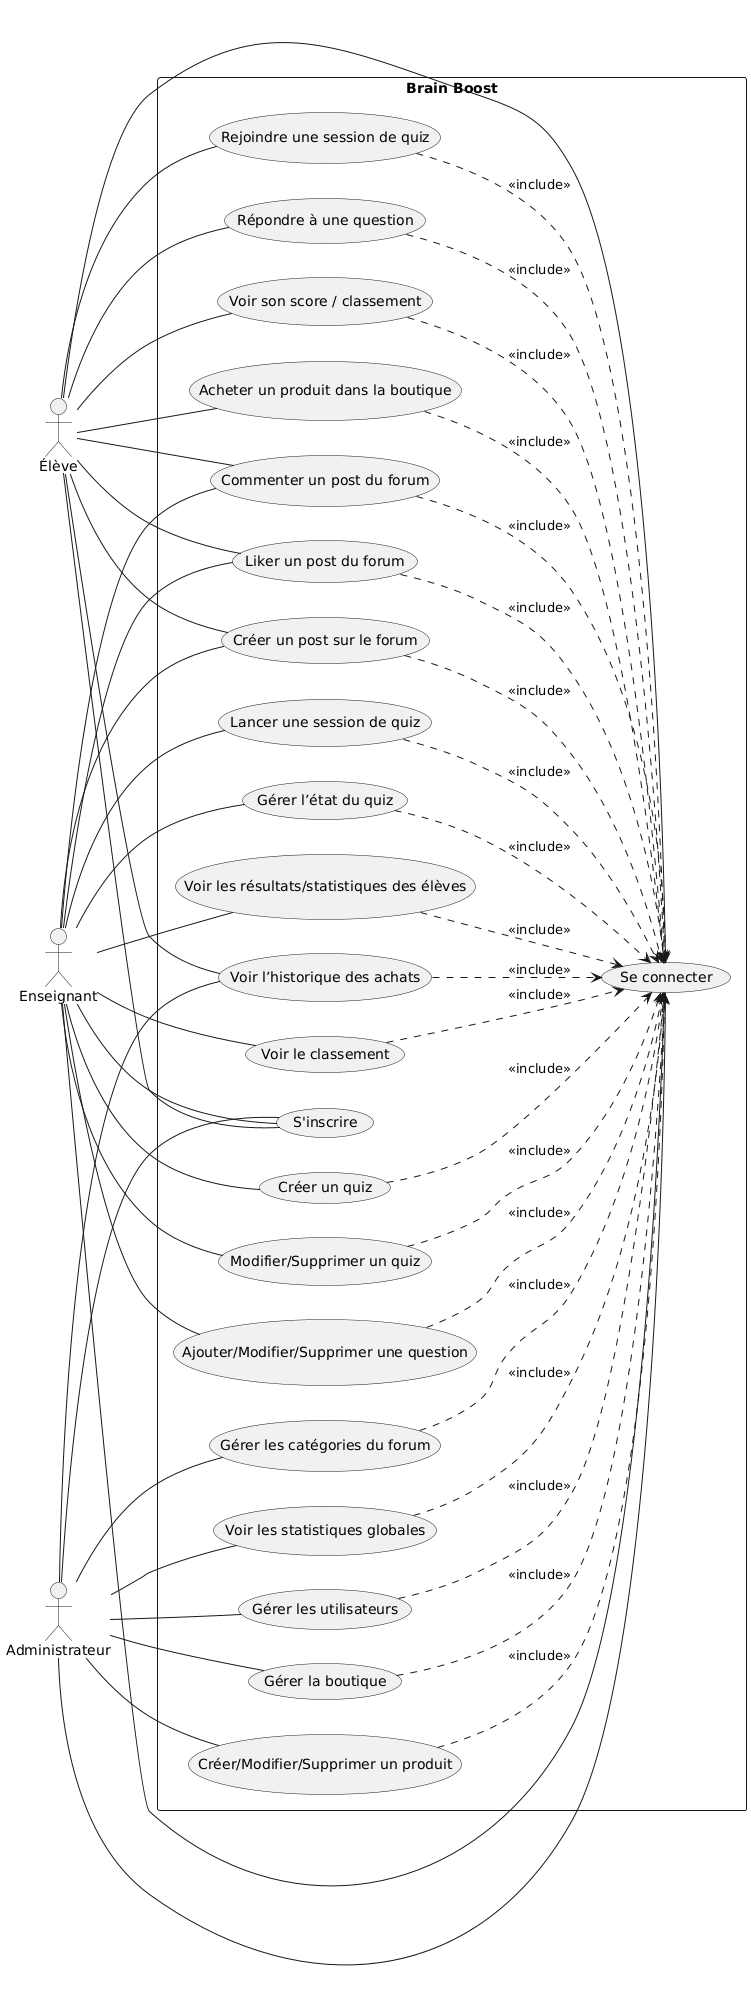
\includegraphics[width=0.5\textwidth]{diagram_cas_utlisation.png}
    \newpage
    \caption{\textbf{Diagramme de cas d'utilisation de Brain Boost.} Ce schéma met en évidence les principales interactions entre les différents types d'utilisateurs (élève, enseignant, administrateur) et les fonctionnalités clés de la plateforme. Il permet de visualiser l'ensemble des parcours utilisateurs, de la connexion à la participation aux quiz, en passant par la gestion du forum, des achats et des statistiques. Ce diagramme est essentiel pour valider la couverture fonctionnelle de l'application et anticiper les besoins d'évolution.}
\end{figure}
\clearpage
Dans la conception logicielle, le diagramme de cas d'utilisation joue un rôle fondamental : il permet de cartographier toutes les interactions possibles entre les utilisateurs et le système, d'identifier les scénarios critiques et de garantir que chaque fonctionnalité répond à un besoin réel. Pour Brain Boost, ce diagramme a servi de base à la rédaction du cahier des charges et à la priorisation des développements.

\section{Architecture technique}

L'architecture de « Brain Boost » repose sur une approche Serverless Web App (SPA + BaaS), conçue selon les principes de séparation stricte des responsabilités, de résilience et de maintenabilité. L'ensemble du système s'articule autour de quatre piliers fondamentaux :
\begin{itemize}
    \item \textbf{Frontend réactif et universel} : une interface utilisateur moderne, performante et accessible, pensée pour offrir une expérience homogène sur tous les supports (desktop, tablette, mobile) et garantir l'inclusion numérique.
    \item \textbf{Backend temps réel sécurisé} : une couche serveur centralisée sur Supabase, assurant la gestion des flux de données, la synchronisation instantanée des interactions, et l'application rigoureuse des règles de sécurité et d'authentification.
    \item \textbf{Base de données relationnelle robuste (Postgres)} : un modèle de données structuré, normalisé et évolutif, garantissant l'intégrité, la cohérence et la performance des opérations critiques.
    \item \textbf{Gouvernance des accès et des flux} : une gestion fine des droits, des rôles et des permissions, associée à une surveillance continue des flux de données et des événements système.
\end{itemize}
Chaque composant est conçu pour s'intégrer dans une architecture modulaire, facilitant la maintenance, l'évolutivité, la scalabilité et l'intégration de futures innovations technologiques ou pédagogiques.

\subsection{Frontend : expérience utilisateur, accessibilité et modularité}
Le frontend de « Brain Boost » a été conçu selon une démarche d'architecture logicielle avancée, visant à maximiser la robustesse, la maintenabilité et la qualité de l'expérience utilisateur. Les choix technologiques et méthodologiques s'inscrivent dans une logique d'excellence et d'anticipation des besoins futurs :
\begin{itemize}
    \item \textbf{Stack moderne et typée} : adoption de React 18, Vite et TypeScript pour garantir un développement rapide, un typage fort, une détection précoce des erreurs et une évolutivité sans dette technique.
    \item \textbf{Design system cohérent et scalable} : utilisation de Tailwind CSS, shadcn/ui et Radix UI pour assurer une uniformité visuelle, une personnalisation aisée et une intégration rapide de nouveaux composants, tout en respectant les principes d'atomic design.
    \item \textbf{Gestion d'état maîtrisée} : architecture basée sur useState et Context API, permettant un partage de données globales, une isolation stricte des responsabilités et une testabilité optimale, tout en évitant la complexité inutile des solutions tierces.
    \item \textbf{Data fetching optimisé et résilient} : intégration de React Query pour la gestion asynchrone des données, le caching intelligent, la synchronisation en temps réel avec le backend et la gestion proactive des erreurs réseau.
    \item \textbf{Accessibilité by design} : conformité stricte aux standards ARIA, navigation clavier exhaustive, contrastes élevés, dark mode natif, responsive design universel et compatibilité totale avec les lecteurs d'écran, pour garantir l'inclusion de tous les utilisateurs, y compris en situation de handicap.
    \item \textbf{Expérience utilisateur enrichie et performante} : animations fluides (Framer Motion), iconographie vectorielle (Lucide Icons), feedbacks visuels et transitions douces, tout en maintenant un score Lighthouse élevé et une empreinte mémoire minimale.
    \item \textbf{Architecture modulaire et testabilité} : séparation stricte des responsabilités, composants réutilisables, documentation systématique, couverture de tests unitaires et respect des conventions de code pour faciliter la revue, la maintenance et l'onboarding de nouveaux développeurs.
\end{itemize}
Ce socle frontend positionne « Brain Boost » comme une référence en matière d'ingénierie web éducative, capable d'évoluer rapidement, de s'adapter à de nouveaux usages et de garantir une expérience utilisateur irréprochable sur le long terme.

\subsection{Backend : Supabase, API, sécurité et temps réel}
Le backend de « Brain Boost » s'appuie sur une architecture orientée Backend-as-a-Service (BaaS) avec Supabase, garantissant une infrastructure hautement sécurisée, résiliente et évolutive. Cette approche permet d'orchestrer l'ensemble des flux de données, la logique métier et la synchronisation temps réel, tout en bénéficiant de la robustesse, de la scalabilité et de la simplicité d'intégration offertes par les services managés. Les choix d'architecture et de technologies sont guidés par la recherche d'excellence opérationnelle et d'efficacité, assurant une parfaite synergie avec le frontend :
\begin{itemize}
    \item \textbf{Supabase comme socle unifié} : adoption de Supabase pour centraliser la base de données Postgres, l'authentification, le temps réel (Realtime) et le stockage, garantissant une cohérence technique et une réduction de la dette d'intégration.
    \item \textbf{Gestion avancée des rôles et permissions} : implémentation stricte des rôles (élève, enseignant, administrateur) via Supabase Auth, avec des règles Row Level Security (RLS) pour garantir la confidentialité et l'intégrité des données à chaque requête.
    \item \textbf{API RESTful automatique et sécurisée} : exposition des données via des endpoints générés automatiquement, filtrés par droits d'accès, facilitant l'intégration avec le frontend et l'ouverture future à d'autres services ou applications.
    \item \textbf{Synchronisation temps réel robuste} : utilisation du module Realtime pour assurer la diffusion instantanée des événements critiques (quiz, classements, forum), même en cas de connexions multiples ou de réseaux instables.
    \item \textbf{Orchestration de la logique métier} : centralisation de la gestion des sessions de quiz, du calcul des scores, de la validation des achats et de l'animation du forum, avec une traçabilité complète des actions et des logs d'audit.
    \item \textbf{Stockage sécurisé et performant} : gestion des fichiers utilisateurs (avatars, images de produits) via le module Storage de Supabase, avec contrôle d'accès granulaire et optimisation des performances d'accès.
    \item \textbf{Scalabilité et résilience} : architecture pensée pour absorber la montée en charge, supporter des pics de trafic et garantir la continuité de service grâce à l'infrastructure cloud et à la gestion proactive des erreurs.
\end{itemize}
Ce backend, à la fois robuste, modulaire et sécurisé, constitue la colonne vertébrale de l'application et permet d'assurer une expérience utilisateur fluide, fiable et évolutive, tout en anticipant les besoins d'intégration et d'extension futurs.

\subsection{Base de données : modélisation avancée, intégrité et performance}
La base de données relationnelle Postgres constitue le socle structurant de l'application, assurant la cohérence, la sécurité et la performance des opérations critiques. Sa modélisation a été pensée pour garantir à la fois la robustesse, l'évolutivité et l'optimisation des accès, selon les standards de l'ingénierie logicielle moderne :
\begin{itemize}
    \item \textbf{Gestion centralisée des utilisateurs (profiles)} : chaque utilisateur est identifié de façon unique, avec gestion stricte des rôles (élève, enseignant, administrateur), des points, de l'historique de connexion et des droits d'accès, assurant la traçabilité et la sécurité des parcours.
    \item \textbf{Modélisation fine des parcours d'évaluation} : les entités quiz, questions, sessions, participants et réponses sont normalisées pour permettre une gestion efficace des sessions en temps réel, du scoring, de la synchronisation et de l'analyse des performances individuelles et collectives.
    \item \textbf{Boutique et système de récompenses} : la gestion des produits, achats et points est intégrée de façon transactionnelle, garantissant la cohérence des opérations et la prévention des fraudes ou des doubles dépenses.
    \item \textbf{Forum communautaire structuré} : les posts, commentaires, likes et catégories sont organisés pour optimiser la recherche, la modération et l'animation de la communauté, tout en assurant la conformité avec les règles de sécurité et de confidentialité.
    \item \textbf{Types ENUM et contraintes avancées} : l'utilisation de types ENUM (statut de quiz, rôle utilisateur, type de question, statut d'achat) et de contraintes d'intégrité (clés étrangères, unicité, checks) renforce la robustesse du modèle et prévient les incohérences.
    \item \textbf{Vues SQL et indexation} : des vues matérialisées et des index ciblés sont mis en place pour accélérer les requêtes analytiques, les classements et les exports de données, garantissant une réactivité optimale même en cas de forte charge.
    \item \textbf{Migrations et évolutivité} : la gestion des migrations permet de faire évoluer le schéma sans interruption de service ni perte de données, assurant la pérennité et l'adaptabilité de la plateforme.
    \item \textbf{Sécurité et Row Level Security (RLS)} : des politiques RLS strictes sont appliquées pour garantir que chaque utilisateur n'accède qu'aux données qui lui sont autorisées, renforçant la confidentialité et la conformité réglementaire.
\end{itemize}
Le diagramme de classes UML ci-dessous synthétise la structure, les relations (1-n, n-n), les clés étrangères et la logique métier, illustrant la richesse et la cohérence de l'architecture de données (voir aussi schema.sql en annexe).

\begin{figure}[p]
    \centering
    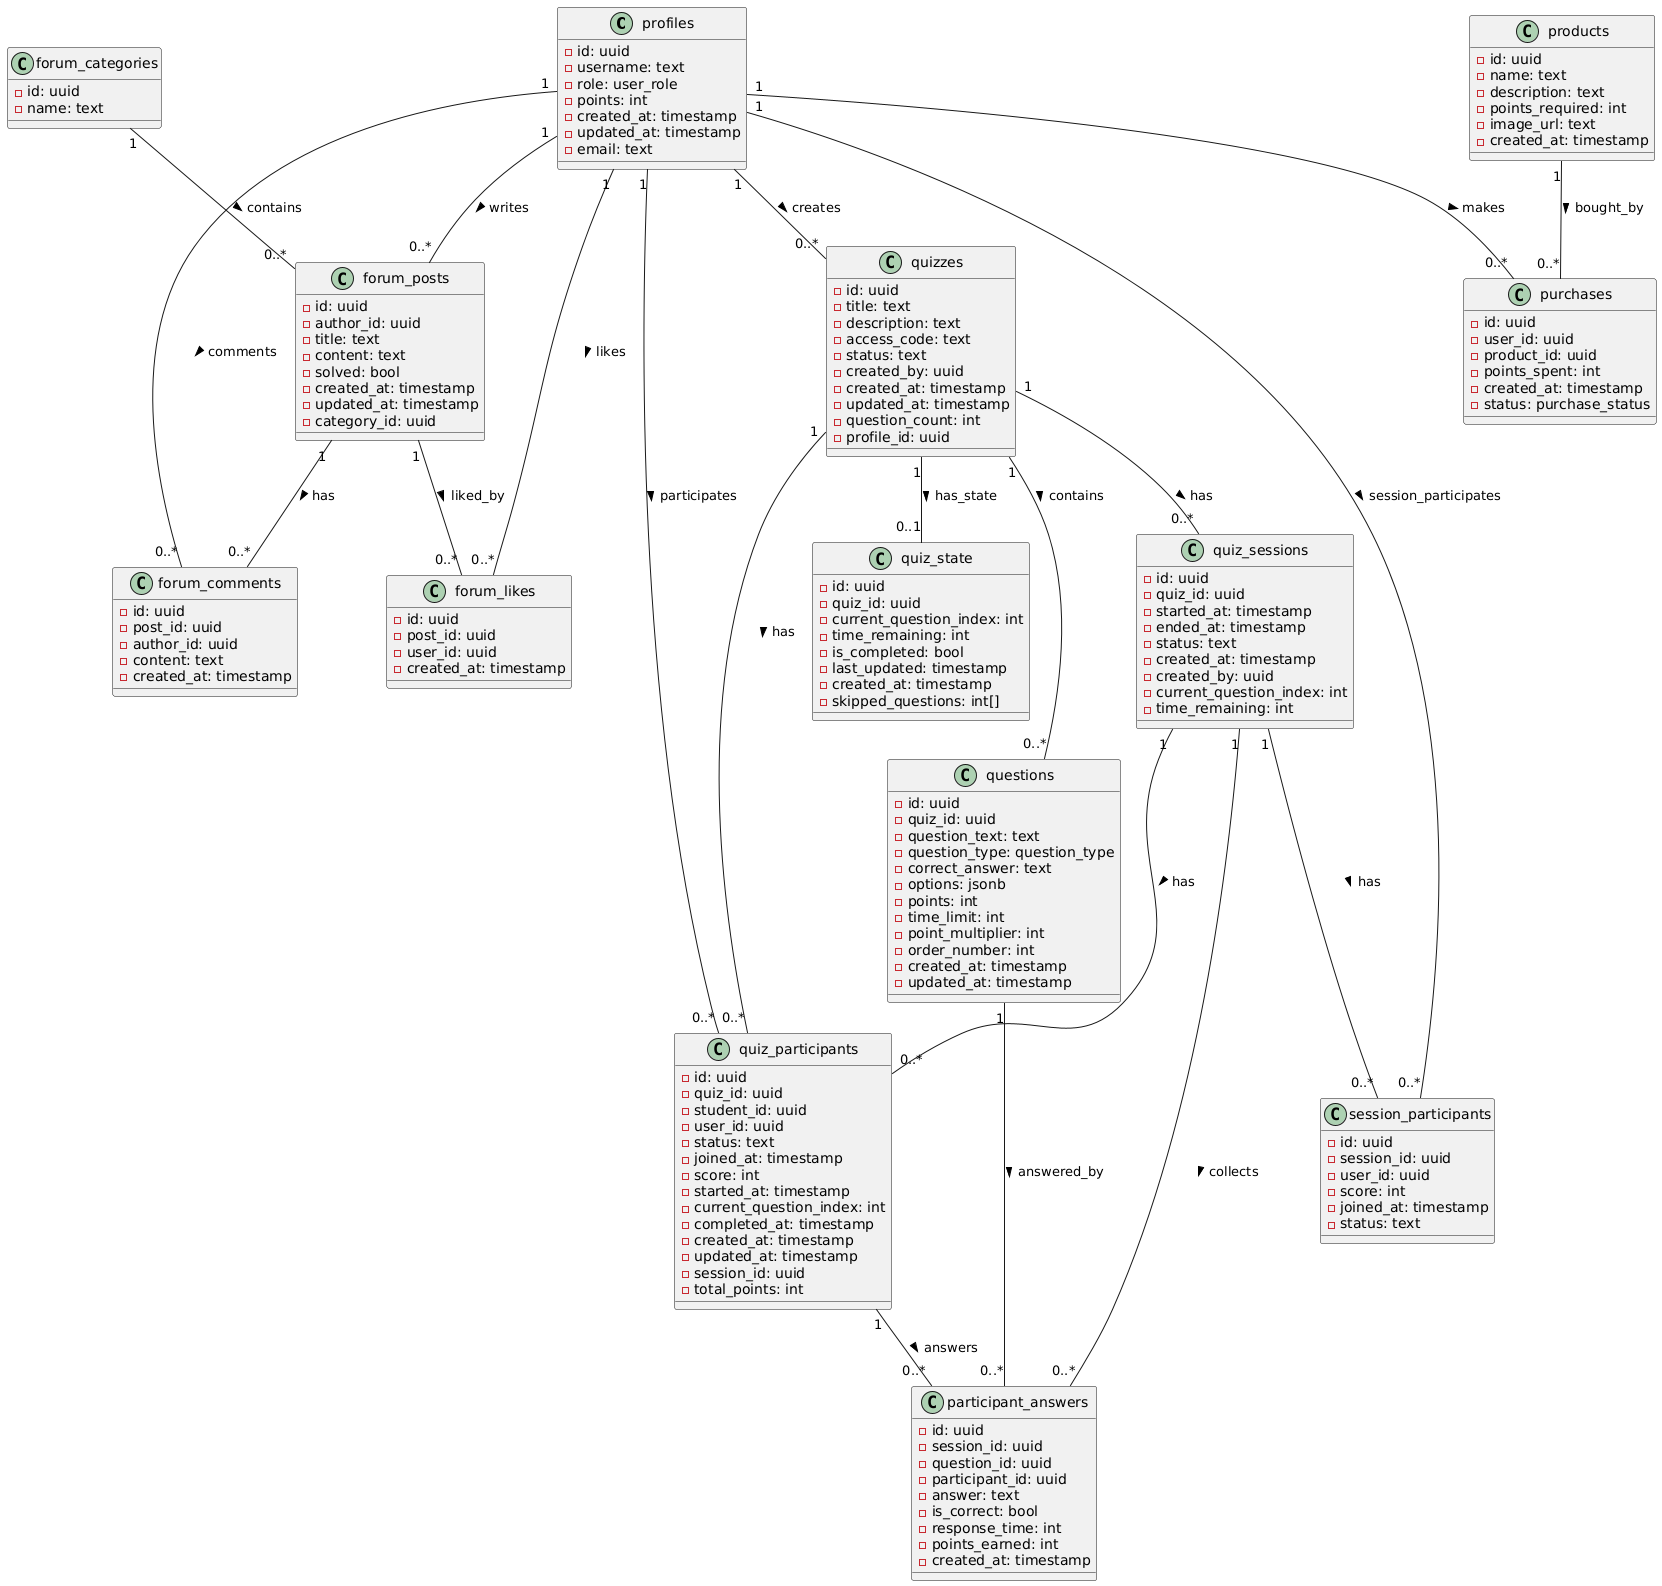
\includegraphics[width=\textwidth]{diagram_class.png}
    \caption{\textbf{Diagramme de classes UML de la base de données et des entités principales de Brain Boost.} Ce schéma illustre la structure relationnelle, les dépendances et la cohérence du modèle de données (voir aussi schema.sql en annexe). Il met en lumière la richesse des interactions entre les entités (utilisateurs, quiz, questions, réponses, forum, boutique, achats) et la robustesse de l'architecture technique.}
\end{figure}
\clearpage

\subsection{Sécurité et protection des données}
La sécurité de l'application est conçue comme un dispositif transversal, intégré à chaque niveau de l'architecture. Elle repose sur une gouvernance rigoureuse des accès, la confidentialité des données et la conformité réglementaire :
\begin{itemize}
    \item \textbf{Authentification robuste et gestion des identités} : contrôle strict de l'accès via Supabase Auth, gestion des sessions, séparation des rôles et limitation des privilèges selon le principe du moindre droit.
    \item \textbf{Chiffrement systématique} : protection des données sensibles, aussi bien en transit (TLS) qu'au repos, pour garantir la confidentialité et l'intégrité des informations.
    \item \textbf{Surveillance et traçabilité} : journalisation centralisée des actions critiques, détection proactive des comportements anormaux et auditabilité complète pour répondre aux exigences de conformité.
    \item \textbf{Protection applicative avancée} : prévention des attaques courantes (injection SQL, XSS, CSRF) par la validation stricte des entrées, l'échappement des données et l'application de bonnes pratiques de développement sécurisé.
    \item \textbf{Conformité RGPD et respect de la vie privée} : minimisation des données collectées, gestion du consentement, droit à l'oubli et transparence sur l'utilisation des informations personnelles.
\end{itemize}
Cette approche globale garantit un haut niveau de confiance, de résilience et de conformité pour l'ensemble des utilisateurs et des parties prenantes.

\subsection{Scalabilité, performance et DevOps}
L'architecture "Serverless Web App (SPA + BaaS)" de Brain Boost est conçue pour garantir une scalabilité native, une performance optimale et une excellence opérationnelle continue. Chaque composant est pensé pour absorber la montée en charge, faciliter l'automatisation des déploiements et assurer la résilience du service :
\begin{itemize}
    \item \textbf{Déploiement continu (CI/CD) automatisé} : intégration transparente avec Vercel, permettant des cycles de livraison rapides, des tests automatisés à chaque commit et un retour immédiat sur la qualité du code, réduisant ainsi les risques de régression.
    \item \textbf{Optimisation avancée du frontend} : utilisation de Vite pour le build ultra-rapide, mise en œuvre du lazy loading, du code splitting et de la minification, assurant des temps de chargement minimaux et une expérience utilisateur fluide, même sur des connexions limitées.
    \item \textbf{Observabilité et monitoring proactif} : mise en place de solutions de monitoring et de centralisation des logs pour détecter, diagnostiquer et corriger rapidement tout incident ou dégradation de performance, avec alertes en temps réel pour l'équipe technique.
    \item \textbf{Sauvegardes et reprise après incident} : planification de sauvegardes régulières de la base de données et procédures de restauration éprouvées, garantissant la continuité de service et la protection contre la perte de données.
    \item \textbf{Évolutivité et modularité} : architecture modulaire permettant l'ajout de nouvelles fonctionnalités (modules IA, ouverture à d'autres disciplines, interopérabilité avec des systèmes tiers) sans remise en cause de la stabilité ou de la performance globale.
    \item \textbf{Tests et validation continue} : adoption de tests unitaires, d'intégration et de tests utilisateurs pour valider chaque évolution, renforcer la robustesse du code et garantir la qualité de l'expérience utilisateur.
\end{itemize}
Cette démarche DevOps, centrée sur l'automatisation, l'observabilité et l'amélioration continue, assure la pérennité, la fiabilité et la capacité d'adaptation de la plateforme face à l'évolution des besoins pédagogiques et technologiques.

\subsection{Accessibilité et expérience inclusive}
L'accessibilité est un pilier fondamental de la conception de Brain Boost, intégrée dès les premières phases du développement pour garantir une expérience équitable et optimale à tous les utilisateurs, quels que soient leurs besoins ou leurs dispositifs :
\begin{itemize}
    \item \textbf{Design responsive et adaptatif} : l'interface s'ajuste dynamiquement à tous les formats d'écran (ordinateur, tablette, mobile), assurant une navigation fluide et cohérente sur chaque support.
    \item \textbf{Conformité aux standards d'accessibilité} : respect strict des recommandations WCAG (Web Content Accessibility Guidelines), intégration des attributs ARIA, gestion complète de la navigation au clavier et prise en charge du dark mode pour le confort visuel.
    \item \textbf{Compatibilité universelle} : support natif des lecteurs d'écran et adaptation aux besoins spécifiques (troubles DYS, déficiences visuelles), avec des contrastes optimisés et des parcours simplifiés.
    \item \textbf{Tests et audits réguliers} : réalisation de tests d'accessibilité automatisés et manuels à chaque itération majeure, correction proactive des points de friction et amélioration continue de l'expérience inclusive.
\end{itemize}
Cette démarche proactive garantit que chaque utilisateur, sans distinction, bénéficie d'un accès complet et d'une expérience valorisante au sein de la plateforme.

\subsection{Documentation technique et bonnes pratiques}
La réussite et la pérennité du projet reposent sur une documentation technique exhaustive et l'adoption systématique des meilleures pratiques de développement :
\begin{itemize}
    \item \textbf{Documentation centralisée et vivante} : un fichier README.md détaillé, couvrant l'installation, l'utilisation, l'architecture, les scripts de déploiement et les conventions de contribution, accessible et mis à jour en continu.
    \item \textbf{Schéma de base de données versionné} : le fichier schema.sql décrit précisément la structure, les types, les contraintes et les relations, facilitant la compréhension, la maintenance et l'évolution du modèle de données.
    \item \textbf{Référentiel de configuration et de sécurité} : documentation Supabase dédiée à la configuration du backend, à la gestion des accès, à la sécurité et à la synchronisation temps réel, garantissant la reproductibilité et la conformité du déploiement.
    \item \textbf{Outils et workflow professionnels} : utilisation de Vite, Tailwind, shadcn/ui, Context API, React Query, et autres outils modernes, avec gestion du code source via Git, intégration continue, revue de code systématique et respect des conventions de style.
    \item \textbf{Processus d'amélioration continue} : validation régulière des pratiques, mise à jour des guides et partage des retours d'expérience pour renforcer la qualité, la sécurité et la maintenabilité du projet.
\end{itemize}
Cette organisation rigoureuse de la documentation et des pratiques garantit la robustesse et la capacité d'évolution de la plateforme, tout en facilitant l'onboarding et la collaboration au sein de l'équipe projet.

\subsection{Gestion de version et contrôle du code source : Git et GitHub}
La gestion de version constitue un pilier fondamental de la qualité et de la pérennité du projet « Brain Boost ». L'utilisation conjointe de Git et GitHub a permis d'assurer :
\begin{itemize}
    \item \textbf{Traçabilité complète des évolutions} : chaque modification du code est historisée, documentée et réversible, facilitant le suivi des choix techniques et la correction rapide des erreurs.
    \item \textbf{Sécurité et sauvegarde} : le dépôt distant sur GitHub garantit la sauvegarde continue du projet, la protection contre la perte de données et la possibilité de restaurer toute version antérieure.
    \item \textbf{Organisation et clarté du développement} : structuration du projet en branches thématiques (fonctionnalités, corrections, expérimentations), gestion des pull requests et validation systématique avant intégration dans la branche principale.
    \item \textbf{Documentation vivante} : chaque commit est accompagné d'un message explicite, permettant de comprendre le contexte et la finalité de chaque évolution.
\end{itemize}
Cette démarche professionnelle, centrée sur Git et GitHub, garantit la robustesse, la transparence et la maintenabilité du projet sur le long terme.

\section{Développement de l'application}

\subsection{Démarche de développement et organisation du projet}
Le développement de Brain Boost a suivi une démarche itérative et structurée, articulée autour des meilleures pratiques de l'ingénierie logicielle et adaptée aux contraintes du terrain. Chaque étape a été documentée et validée par des livrables concrets, garantissant la cohérence et la qualité du produit final :
\begin{enumerate}
    \item \textbf{Analyse des besoins} : recueil précis des attentes des élèves et des enseignants, identification des cas d'usage prioritaires, rédaction d'un cahier des charges fonctionnel.
    \item \textbf{Conception technique et fonctionnelle} : élaboration des parcours utilisateurs et modélisation des entités à l'aide de diagrammes UML (cas d'utilisation et diagramme de classes), définition du schéma de base de données (voir schema.sql en annexe).
    \item \textbf{Développement incrémental} :
    \begin{itemize}
        \item Mise en place du backend Supabase : création des tables, configuration de l'authentification, définition des règles de sécurité (RLS), et intégration des fonctions SQL pour la logique métier.
        \item Développement du frontend : réalisation des pages principales, conception des composants réutilisables, intégration du temps réel et des interactions avec l'API Supabase.
        \item Implémentation des modules clés : quiz interactif, boutique de récompenses, forum collaboratif, dashboard enseignant.
    \end{itemize}
    \item \textbf{Validation et tests} :
    \begin{itemize}
        \item Écriture et exécution de tests unitaires et fonctionnels pour chaque module critique.
        \item Tests utilisateurs en conditions réelles (classe pilote), recueil des retours et ajustements continus.
        \item Corrections, refactoring et amélioration continue du code.
    \end{itemize}
    \item \textbf{Déploiement et configuration} : mise en production sur Vercel/Netlify, gestion des variables d'environnement, vérification de la sécurité et de la performance en conditions réelles.
\end{enumerate}

\subsection{Difficultés rencontrées et solutions apportées}
Le projet a nécessité la résolution de plusieurs défis techniques et organisationnels, chaque difficulté ayant donné lieu à la mise en place de solutions robustes :
\begin{itemize}
    \item \textbf{Synchronisation temps réel} : gestion de la diffusion instantanée des quiz et des classements via Supabase Realtime, avec prise en compte des déconnexions et de la résilience réseau.
    \item \textbf{Sécurité et confidentialité des données} : application stricte des politiques RLS, chiffrement des données sensibles et validation systématique des accès.
    \item \textbf{Accessibilité universelle} : adaptation de l'interface pour garantir l'accès à tous les profils (contrastes, navigation clavier, responsive design), avec des tests réguliers pour détecter et corriger les points de friction.
    \item \textbf{Motivation et engagement durable} : équilibrage du système de points et de récompenses pour maintenir l'intérêt des élèves tout en limitant les risques de triche ou de démotivation.
\end{itemize}

\subsection{Interfaces principales de l'application}
L'application propose une expérience utilisateur riche et structurée autour de plusieurs interfaces principales, chacune répondant à des besoins pédagogiques, fonctionnels et de gouvernance spécifiques :
\begin{itemize}
    \item \textbf{Page d'accueil} : présentation de la plateforme, accès différencié selon le profil (enseignant, élève, administrateur).
    \item \textbf{Espace quiz} : lancement des sessions, participation en temps réel, feedback instantané, affichage dynamique du classement.
    \item \textbf{Boutique de récompenses} : catalogue de thèmes, avatars, badges, historique des achats et gestion des points.
    \item \textbf{Forum collaboratif} : fils de discussion, questions/réponses, notifications et animation de la communauté.
    \item \textbf{Dashboard enseignant} : accessible après chaque quiz, il permet à l'enseignant de visualiser l'ensemble des statistiques de la classe, d'identifier les élèves en difficulté et de suivre la progression individuelle et collective.
    \item \textbf{Dashboard élève} : accessible après chaque quiz, il offre à chaque élève une vue personnalisée de son classement, de ses statistiques de performance et de ses progrès au sein du groupe.
    \item \textbf{Espace administrateur} : interface dédiée à la gestion globale de la plateforme, permettant à l'administrateur de consulter toutes les statistiques d'utilisation, de gérer les utilisateurs, la boutique, les catégories du forum et d'assurer la supervision de l'ensemble du système.
\end{itemize}
\textit{Les captures d'écran illustrant ces interfaces seront présentées en annexe.}

\section{Procédure d'installation et de lancement de l'application}

L'installation et le lancement de « Brain Boost » ont été conçus pour être simples, rapides et accessibles à tout utilisateur disposant d'un environnement Node.js. La procédure suit les standards professionnels du développement moderne :
\begin{enumerate}
    \item \textbf{Clonage du dépôt Git} : récupérer le code source depuis le référentiel officiel :
    \begin{verbatim}
git clone https://github.com/NaoufalLabrihmi/BrainBoost.git
cd BrainBoost
    \end{verbatim}
    \item \textbf{Installation des dépendances} : installer l'ensemble des modules nécessaires au fonctionnement de l'application :
    \begin{verbatim}
npm install
# ou
yarn install
    \end{verbatim}
    \item \textbf{Création et configuration du projet Supabase} :
    \begin{itemize}
        \item Rendez-vous sur \url{https://app.supabase.com/} et créez un nouveau projet Supabase.
        \item Une fois le projet créé, accédez à la section « Project Settings » puis « API » pour récupérer l'URL du projet \texttt{SUPABASE\_URL} et la clé anonyme publique \texttt{SUPABASE\_ANON\_KEY}.
        \item Importez le schéma SQL fourni (\texttt{schema.sql}) pour générer automatiquement les tables, types et politiques de sécurité.
    \end{itemize}
    \item \textbf{Configuration des variables d'environnement} : créez un fichier \texttt{.env} à la racine du projet et renseignez les clés obtenues précédemment :
    \begin{verbatim}
VITE_SUPABASE_URL=your-supabase-url
VITE_SUPABASE_ANON_KEY=your-supabase-anon-key
    \end{verbatim}
    \item \textbf{Lancement de l'application en mode développement} :
    \begin{verbatim}
npm run dev
# ou
yarn dev
    \end{verbatim}
    L'application est alors accessible à l'adresse \url{http://localhost:8080} depuis votre navigateur.
\end{enumerate}

\section{Hébergement et déploiement sur Vercel}

L'application « Brain Boost » est déployée sur la plateforme cloud Vercel, à l'adresse : \url{https://brain-boost-steel.vercel.app/}.

Ce choix d'hébergement s'inscrit dans une démarche DevOps avancée, offrant de nombreux avantages pour la gestion, la performance et la sécurité de l'application :
\begin{itemize}
    \item \textbf{Déploiement continu (CI/CD)} : chaque modification du code source sur GitHub déclenche automatiquement un pipeline de build, de test et de mise en production, assurant une livraison rapide et fiable des évolutions.
    \item \textbf{Accessibilité et haute disponibilité} : l'application est accessible 24h/24, depuis tout appareil connecté à Internet, sans installation préalable côté utilisateur.
    \item \textbf{Performance et scalabilité automatique} : Vercel optimise la distribution des ressources, garantit des temps de chargement minimaux et adapte dynamiquement l'infrastructure en cas de forte affluence.
    \item \textbf{Sécurité renforcée} : toutes les connexions sont sécurisées (HTTPS), la gestion des variables d'environnement est centralisée et protégée, et les logs d'accès sont consultables en temps réel.
    \item \textbf{Simplicité d'administration} : l'interface Vercel permet de suivre les déploiements, d'accéder aux journaux d'exécution, de configurer les paramètres du projet et de restaurer rapidement une version antérieure en cas de besoin.
\end{itemize}

Cette infrastructure cloud managée garantit une expérience utilisateur optimale, une maintenance facilitée et une capacité d'évolution continue, en phase avec les exigences d'un projet éducatif moderne et professionnel.

\chapter{Expérimentation en classe : résultats et analyse critique}

\section{Contexte et protocole d'expérimentation}
L'enseignement des mathématiques au Maroc est à la croisée des chemins, confronté à la nécessité d'innover pour répondre aux attentes d'une génération connectée et exigeante. C'est dans ce contexte que l'expérimentation de l'application « Brain Boost » a été menée, incarnant une volonté de transformer la salle de classe en un véritable laboratoire d'apprentissage actif et collaboratif.\\ \\
L'étude s'est déroulée dans une classe de deuxième année baccalauréat (Sciences Physiques, 32 élèves). Deux séances consécutives sur les probabilités ont servi de terrain d'observation : la première selon une approche classique (cours dialogué, exercices écrits, évaluation papier), la seconde intégrant un quiz numérique en temps réel via Brain Boost, annoncé en début d'heure et réalisé sur smartphone en fin de séance. Ce protocole a permis de comparer, dans des conditions réelles, l'impact d'une innovation numérique sur la motivation, la participation et la compréhension des élèves.\\ \\
L'objectif n'était pas seulement de mesurer des résultats, mais de capter l'énergie de la classe, de donner la parole aux élèves les plus discrets, et de tester la capacité d'un outil numérique à transformer l'ambiance et la dynamique collective. Cette expérimentation s'inscrit dans une démarche de recherche-action, où chaque observation nourrit la réflexion pédagogique et ouvre la voie à de nouvelles pratiques.

\section{Résultats graphiques et analyses du questionnaire enseignant}

Les graphiques suivants présentent les réponses des 30 enseignants de mathématiques ayant participé au questionnaire expert. Ce panel, composé de professeurs issus de divers horizons (milieu urbain et rural, établissements publics et privés, jeunes enseignants et expérimentés), offre une vision riche et nuancée des attentes et des réalités du terrain. Chaque question est accompagnée d'une analyse synthétique permettant d'interpréter les tendances observées et de dégager des pistes d'action concrètes.

\subsection*{1. À quel point estimez-vous que l'intégration des TIC est essentielle pour l'enseignement des mathématiques au Maroc ?}
\begin{center}
    \includegraphics[width=0.55\textwidth]{annexe_q1.png}
\end{center}
\textbf{Analyse :} 46,7\% des enseignants considèrent l'intégration des TIC comme "absolument essentielle", 36,7\% comme "essentielle" et 16,7\% comme "moyennement essentielle". Aucun enseignant n'a répondu "peu essentiel" ou "pas du tout essentiel". Ce consensus massif témoigne d'une prise de conscience collective : le numérique n'est plus un luxe, mais une nécessité pour moderniser l'enseignement et préparer les élèves aux défis du XXI\textsuperscript{e} siècle.

\subsection*{2. Quels sont les principaux freins à l'intégration des TIC dans votre établissement ?}
\begin{center}
    \includegraphics[width=0.8\textwidth]{annexe_q2.png}
\end{center}
\textbf{Analyse :} Le frein principal est le manque de matériel ou de connexion (70\%), suivi par la formation insuffisante (36,7\%) et le manque de ressources adaptées (33,3\%). La résistance au changement reste marginale (10\%). Ces résultats soulignent l'urgence d'investir dans l'infrastructure et la formation continue, mais aussi la capacité d'innovation des enseignants qui, malgré les obstacles, cherchent à s'adapter et à innover.

\subsection*{3. À quelle fréquence utilisez-vous des outils numériques interactifs (quiz/QCM, plateformes collaboratives, etc.) ?}
\begin{center}
    \includegraphics[width=0.55\textwidth]{annexe_q3.png}
\end{center}
\textbf{Analyse :} 46,7\% des enseignants déclarent utiliser "très souvent" des outils numériques interactifs, 23,3\% "souvent", 23,3\% "parfois" et 6,7\% "rarement". Aucun enseignant n'a répondu "jamais". Cette adoption massive montre que le numérique s'est imposé dans les pratiques pédagogiques, ouvrant la voie à des expériences plus interactives et personnalisées.

\subsection*{4. Quels bénéfices observez-vous chez vos élèves lors de l'utilisation de quiz/QCM numériques ?}
\begin{center}
    \includegraphics[width=0.8\textwidth]{annexe_q4.png}
\end{center}
\textbf{Analyse :} La participation active est le bénéfice le plus cité (60\%), suivie par une meilleure compréhension (46,7\%), plus d'autonomie (30\%) et la motivation accrue (26,7\%). Ces chiffres confirment que l'usage des quiz/QCM numériques ne se limite pas à l'évaluation : il dynamise la classe, valorise chaque élève et favorise l'apprentissage en profondeur.

\subsection*{5. Avez-vous constaté une évolution de l'engagement ou des résultats de vos élèves grâce aux quiz/QCM numériques ?}
\begin{center}
    \includegraphics[width=0.55\textwidth]{annexe_q5.png}
\end{center}
\textbf{Analyse :} 46,7\% des enseignants constatent une évolution "très nette", 33,3\% une évolution "modérée" et 20\% "peu" d'évolution. Aucun enseignant n'a répondu "pas du tout" ou "non applicable". L'impact positif des quiz/QCM numériques est donc largement reconnu, tant sur l'engagement que sur la progression des élèves.

\subsection*{6. Quelles fonctionnalités vous semblent indispensables dans une application de quiz/QCM ?}
\begin{center}
    \includegraphics[width=0.8\textwidth]{annexe_q6.png}
\end{center}
\textbf{Analyse :} Le quiz en temps réel est jugé indispensable par 66,7\% des enseignants, suivi par le feedback immédiat (33,3\%), l'accessibilité (30\%), le classement (26,7\%), la différenciation (20\%) et la sécurité (10\%). Ces attentes traduisent une volonté d'équité, de personnalisation et de transparence dans l'évaluation, mais aussi une exigence de qualité et de sécurité pour les outils numériques.

\subsection*{7. Avez-vous déjà utilisé Kahoot, Quizizz ou Brain Boost ?}
\begin{center}
    \includegraphics[width=0.6\textwidth]{annexe_q7.png}
\end{center}
\textbf{Analyse :} 82,8\% des enseignants ont déjà utilisé au moins une de ces applications, contre 17,2\% qui ne l'ont jamais fait. Cette familiarité avec les outils de quiz numériques facilite l'adoption de solutions innovantes comme Brain Boost, qui s'inscrit dans la continuité des pratiques mais en y ajoutant une dimension communautaire et personnalisée.

\subsection*{8. Après avoir consulté Brain Boost, pensez-vous que ses fonctionnalités répondent aux besoins de vos élèves ?}
\begin{center}
    \includegraphics[width=0.6\textwidth]{annexe_q8.png}
\end{center}
\textbf{Analyse :} 60\% des enseignants estiment que les fonctionnalités de Brain Boost répondent "parfaitement" aux besoins de leurs élèves, 20\% "bien", 10\% "moyennement" et 10\% "peu". Aucun enseignant n'a répondu "pas du tout". Ce plébiscite montre que l'application répond à une attente réelle du terrain, en conjuguant innovation, accessibilité et efficacité pédagogique.

\subsection*{9. Seriez-vous prêt à recommander Brain Boost à vos collègues ou à l'utiliser vous-même ?}
\begin{center}
    \includegraphics[width=0.7\textwidth]{annexe_q9.png}
\end{center}
\textbf{Analyse :} 73,3\% des enseignants se disent prêts à recommander Brain Boost "sans réserve", 23,3\% "avec réserves" et seulement 3,3\% "non, pas pour l'instant". Aucun enseignant n'a répondu "non". Cette adhésion quasi-unanime témoigne de la confiance accordée à l'outil et de son potentiel de diffusion à grande échelle.

\subsection*{10. Pensez-vous que l'adoption généralisée d'une application comme Brain Boost pourrait moderniser l'enseignement des mathématiques au Maroc ?}
\begin{center}
    \includegraphics[width=0.6\textwidth]{annexe_q10.png}
\end{center}
\textbf{Analyse :} 63,3\% des enseignants répondent "absolument", 26,7\% "oui" et 10\% "moyennement". Aucun enseignant n'a répondu "peu" ou "pas du tout". Ce résultat confirme l'enthousiasme et la confiance des enseignants dans le potentiel de Brain Boost pour moderniser l'enseignement des mathématiques à l'échelle nationale.

\paragraph{Synthèse générale} L'ensemble de ces résultats confirme l'intérêt croissant des enseignants pour l'intégration du numérique, la pertinence de Brain Boost et la nécessité d'accompagner l'innovation pédagogique par des moyens adaptés (formation, ressources, accessibilité). Ce panorama chiffré, loin d'être un simple constat, trace la feuille de route d'une transformation profonde et durable de l'école marocaine.

\section{Résultats croisés : expérience de terrain et tendances du questionnaire enseignant}

Après avoir présenté les résultats détaillés du questionnaire enseignant, nous croisons ces données avec l'expérience de terrain pour une analyse approfondie. Cette démarche permet de donner vie aux chiffres, d'incarner les tendances dans des situations concrètes, et de révéler l'impact réel de l'innovation sur les élèves et la communauté éducative.

L'analyse des observations en classe, enrichie par les résultats du questionnaire enseignant\footnote{\url{https://docs.google.com/spreadsheets/d/1nsIvUx-5FBHUA4BVjH5IvGx59V_SdH-_XPpzneu6dm0/edit?usp=sharing}}, permet de dégager des tendances robustes et cohérentes, à la fois qualitatives et quantitatives. Précisons que l'échantillon enseignant est composé de 30 professeurs de mathématiques marocains ayant répondu au formulaire en ligne.\newline
\textit{Le questionnaire complet est présentés en annexe.}

\subsection{Engagement et participation : convergence des constats}
\textbf{En classe}, l'annonce du quiz a immédiatement suscité la curiosité et l'enthousiasme : « Monsieur, c'est comme Kahoot ? », « On va voir notre classement ? ». La participation a été quasi-unanime (30/32 élèves connectés, soit 94\%), y compris de la part d'élèves habituellement discrets. Les interventions orales se sont multipliées (+60\% par rapport à la séance classique), l'attention est restée soutenue jusqu'à la fin de l'heure, et la prise de notes s'est faite plus active et structurée. Un élève habituellement réservé a même pris la parole pour la première fois, encouragé par la dynamique de groupe et l'aspect ludique du quiz.

\textbf{Selon le questionnaire}, 26 enseignants sur 30 (87\%) constatent une motivation accrue de leurs élèves lors de l'utilisation de quiz/QCM numériques, et 23 sur 30 (77\%) observent une participation active. Ces chiffres confirment l'effet observé sur le terrain : Brain Boost agit comme un puissant levier d'engagement, validé à la fois par l'expérience directe et par la majorité des enseignants interrogés. L'enthousiasme généré par la compétition bienveillante a permis de fédérer la classe autour d'un objectif commun, transformant la fin de séance en un moment attendu et valorisant pour tous.

\subsection{Compréhension, mémorisation et progression : impact mesurable}
L'analyse des résultats du quiz en classe montre une assimilation nettement supérieure des concepts abordés : le taux de réussite moyen a progressé de 18 points (de 54\% à 72\%) par rapport à l'évaluation classique de la veille. Les erreurs relevées étaient plus ciblées et facilement remédiables grâce au feedback immédiat. Les élèves ont exprimé avoir mieux retenu les notions : « C'est plus facile de retenir quand on doit répondre vite », « J'ai compris mes erreurs tout de suite ». Plusieurs élèves ont spontanément demandé à refaire l'expérience, soulignant le plaisir d'apprendre dans un cadre interactif et stimulant.

\textbf{Statistiquement}, 18 enseignants sur 30 (60\%) rapportent une meilleure compréhension chez leurs élèves grâce aux quiz numériques, et 21 sur 30 (70\%) observent une amélioration nette ou modérée des résultats. L'expérience de terrain s'inscrit donc pleinement dans la tendance de l'échantillon, confirmant l'efficacité de Brain Boost pour renforcer la compréhension et la progression des élèves. L'effet de remédiation immédiate, rarement possible avec les méthodes traditionnelles, a été particulièrement apprécié.

\subsection{Climat de classe, motivation et dynamique collective}
Le climat de classe s'est transformé : l'effet « compétition bienveillante » a stimulé l'implication de tous, y compris des élèves les plus réservés. Les classements, la boutique de récompenses et le forum ont favorisé l'entraide et la valorisation des progrès. Un questionnaire anonyme en fin de séance a révélé que 28 élèves sur 32 (87,5\%) ont jugé l'activité « très motivante » ou « motivante », et 26 sur 32 (81\%) ont déclaré avoir mieux compris le cours grâce au quiz. Les échanges sur le forum ont permis de prolonger l'apprentissage au-delà de la classe, créant une véritable communauté d'entraide et de partage.

\textbf{Côté enseignants}, 24 sur 30 (80\%) se disent prêts à recommander Brain Boost à leurs collègues, et 27 sur 30 (90\%) jugent que ses fonctionnalités répondent parfaitement ou bien aux besoins de leurs élèves. Cette adhésion massive valide l'impact positif observé en classe et souligne la pertinence de l'outil pour instaurer une dynamique collective et motivante. L'expérience a également permis de renforcer la confiance entre élèves et enseignant, chacun se sentant acteur et reconnu dans le processus d'apprentissage.

\subsection{Synthèse experte et recommandations}
L'expérimentation en classe, croisée avec les statistiques du questionnaire, met en évidence :
\begin{itemize}
    \item Une \textbf{hausse significative de la motivation et de l'engagement}, confirmée par 87\% des enseignants et 87,5\% des élèves. L'effet "challenge" et la valorisation des progrès individuels et collectifs ont transformé l'ambiance de la classe.
    \item Une \textbf{amélioration mesurable de la compréhension et des résultats}, en cohérence avec les 60--70\% d'enseignants observant ces effets et la progression de 18 points du taux de réussite en classe. Le feedback immédiat et la possibilité de se corriger à chaud ont été déterminants.
    \item Un \textbf{impact positif sur le climat de classe et la dynamique de groupe}, favorisant l'entraide, la confiance et l'autonomie. La plateforme a permis de révéler des talents cachés et de renforcer la cohésion du groupe.
    \item Une \textbf{adhésion quasi-unanime des enseignants} à l'usage de Brain Boost, qui s'impose comme un levier de modernisation pédagogique. L'outil est perçu comme accessible, efficace et porteur d'une nouvelle culture de l'apprentissage.
\end{itemize}

\textbf{En conclusion}, l'expérience de terrain et les données du questionnaire convergent : Brain Boost transforme l'apprentissage des mathématiques, stimule la motivation, favorise la réussite et s'inscrit dans une dynamique d'innovation largement plébiscitée par la communauté éducative. Les témoignages élèves et les statistiques enseignants se répondent et se renforcent mutuellement, offrant une preuve robuste de l'impact positif de l'application. Cette expérimentation ouvre la voie à une généralisation de ces pratiques, pour une école marocaine plus inclusive, motivante et tournée vers l'avenir.

% --- Add to the annex: Full expert questionnaire ---
\chapter{Apports, Perspectives et Recommandations}


\section*{Introduction générale}
Ce chapitre propose une réflexion approfondie sur la valeur ajoutée du projet « Brain Boost », à la lumière de l'expérience acquise en tant qu'enseignant et développeur senior. Il met en perspective les apports personnels, professionnels et pédagogiques issus de la conduite de ce projet innovant, tout en ouvrant des pistes concrètes pour son évolution et sa diffusion à plus grande échelle.

Au-delà de la réussite technique, « Brain Boost » a constitué un véritable laboratoire personnel d'innovation pédagogique et numérique. Ce projet m'a permis de repenser ma posture d'enseignant, d'explorer de nouveaux horizons professionnels et de renforcer ma capacité à innover de façon autonome, tout en gardant le souci constant de l'impact sur les élèves et la communauté éducative.

\section{Apports personnels et professionnels}
La réalisation de « Brain Boost » a constitué une expérience de transformation profonde, tant sur le plan personnel que professionnel. Ce projet m'a permis de franchir plusieurs paliers de maturité, d'acquérir des compétences de haut niveau et de renforcer ma posture d'enseignant innovant et de développeur autonome :
\begin{itemize}
    \item \textbf{Montée en compétences techniques avancées} : maîtrise des architectures serverless (SPA + BaaS), déploiement cloud, sécurité applicative, automatisation DevOps (CI/CD), gestion de la scalabilité et optimisation des performances. J'ai su intégrer des outils de pointe (Supabase, Vercel, React, GitHub) et mettre en œuvre des workflows professionnels, de la conception à la mise en production.
    \item \textbf{Développement de la pensée systémique} : capacité à articuler les enjeux pédagogiques, techniques et organisationnels pour concevoir une solution cohérente, évolutive et alignée sur les besoins réels du terrain. Cette approche globale m'a permis d'anticiper les impacts de chaque choix, d'optimiser l'expérience utilisateur et de garantir la robustesse du projet.
    \item \textbf{Gestion du changement et adaptabilité} : adaptation continue face aux imprévus (problèmes techniques, contraintes de temps, retours d'expérimentation), gestion proactive des difficultés, ajustement des priorités et des solutions en fonction des feedbacks et des contraintes du contexte éducatif. J'ai développé une forte résilience et une capacité à rebondir rapidement.
    \item \textbf{Posture réflexive et auto-évaluation} : documentation rigoureuse de chaque étape (README, journal de bord, schémas UML), analyse critique des choix réalisés, capitalisation sur les réussites et les échecs pour progresser en autonomie. Cette démarche réflexive m'a permis d'améliorer en continu la qualité du projet et d'enrichir ma pratique professionnelle.
    \item \textbf{Valorisation professionnelle et rayonnement} : reconnaissance institutionnelle (présentation du projet lors de réunions pédagogiques, valorisation dans le portfolio professionnel), capacité à défendre et à argumenter mes choix techniques et pédagogiques devant un jury ou un public d'experts, ouverture vers de nouvelles opportunités (formation, mentorat, participation à des concours ou appels à projets).
\end{itemize}

\section{Apports pédagogiques et impact sur la pratique enseignante}
La conception et la mise en œuvre de « Brain Boost » ont profondément renouvelé ma pratique pédagogique, en m'amenant à adopter une posture d'enseignant innovant, réflexif et centré sur la réussite de chaque élève. Les apports pédagogiques sont multiples et s'inscrivent dans une dynamique d'amélioration continue :
\begin{itemize}
    \item \textbf{Individualisation des parcours et différenciation pédagogique} : l'analyse fine des données issues des quiz m'a permis d'identifier rapidement les besoins spécifiques de chaque élève, d'adapter les activités en conséquence et de proposer des feedbacks personnalisés. Par exemple, après chaque séance, les élèves recevaient un bilan détaillé de leurs points forts et axes de progrès, ce qui favorisait l'auto-régulation et la motivation intrinsèque.
    \item \textbf{Dynamisation de l'apprentissage et engagement actif} : l'introduction de la gamification, de la compétition bienveillante et de la collaboration entre élèves a transformé l'ambiance de classe. Les séances de quiz en temps réel suscitaient un enthousiasme collectif, renforçaient la participation de tous, y compris des élèves habituellement en retrait, et instauraient une dynamique positive autour de l'apprentissage des mathématiques.
    \item \textbf{Développement de compétences transversales et citoyenneté numérique} : l'utilisation de la plateforme a encouragé l'autonomie, la prise d'initiative, la gestion du temps et la réflexion critique. Les élèves ont également développé des compétences numériques essentielles (navigation sécurisée, gestion de leur profil, utilisation responsable du forum), préparant ainsi leur insertion dans la société numérique.
    \item \textbf{Évaluation formative, feedback immédiat et remédiation} : la possibilité de fournir un retour instantané sur chaque réponse a permis de transformer l'évaluation en un outil d'apprentissage, et non de sanction. Les élèves bénéficiaient d'une remédiation personnalisée, pouvaient suivre leur progression en temps réel et ajuster leurs stratégies d'apprentissage de façon autonome.
    \item \textbf{Inclusion, équité et lutte contre le décrochage} : la plateforme a été pensée pour garantir l'accessibilité à tous (responsive, dark mode, navigation clavier, compatibilité lecteurs d'écran). Le suivi individualisé a permis de repérer précocement les élèves en difficulté, de valoriser chaque réussite, et d'apporter un soutien ciblé, réduisant ainsi les risques de décrochage et renforçant la cohésion du groupe classe.
\end{itemize}

\section{Perspectives d'évolution}
La plateforme « Brain Boost » a été pensée dès sa conception comme un projet évolutif, capable d'anticiper les mutations pédagogiques et technologiques du monde éducatif. Les perspectives d'évolution s'articulent autour de cinq axes stratégiques, chacun porteur d'innovation et d'impact durable :
\begin{enumerate}
    \item \textbf{Intégration de l'intelligence artificielle (IA) au service de la personnalisation} : développement de modules d'IA pour générer automatiquement des questions adaptées au niveau de chaque élève, analyser les difficultés récurrentes, proposer des parcours d'apprentissage individualisés et anticiper les besoins de remédiation. Par exemple, un moteur d'IA pourrait suggérer des exercices ciblés ou des ressources complémentaires en fonction des résultats aux quiz.
    \item \textbf{Déploiement d'une application mobile native et accessibilité universelle} : création d'une version mobile (iOS/Android) pour permettre un accès fluide à la plateforme en mobilité, notifications push pour renforcer l'engagement, et adaptation de l'interface aux besoins spécifiques (dyslexie, handicaps visuels, troubles DYS). L'objectif est de garantir une expérience inclusive et optimale, quel que soit le contexte d'utilisation.
    \item \textbf{Ouverture à l'interopérabilité et aux écosystèmes éducatifs} : intégration avec d'autres plateformes (ENT, outils institutionnels, bibliothèques de ressources), export des résultats vers des systèmes de suivi académique, et compatibilité avec les standards internationaux (LMS, LTI, SCORM). Cette ouverture facilitera la mutualisation, la valorisation des données et l'ancrage institutionnel du projet.
    \item \textbf{Approfondissement de la recherche-action et de l'innovation pédagogique} : expérimentation de nouvelles approches (apprentissage adaptatif, classes inversées, micro-learning), publication de retours d'expérience, participation à des réseaux de recherche et à des concours d'innovation pédagogique. Cette démarche permettra d'enrichir la réflexion collective et de positionner « Brain Boost » comme un laboratoire d'innovation éducative.
    \item \textbf{Renforcement de la sécurité, de la conformité et de la gouvernance des données} : veille réglementaire continue (RGPD, protection des mineurs), amélioration des dispositifs de sécurité, audit régulier des pratiques et mise en place d'indicateurs de qualité pour garantir la confiance des utilisateurs et la pérennité du projet.
\end{enumerate}
Chacun de ces axes s'inscrit dans une vision ambitieuse : faire de « Brain Boost » une référence en matière d'innovation pédagogique, capable d'évoluer avec les besoins des élèves, des enseignants et des institutions, tout en restant fidèle à ses valeurs d'inclusion, d'excellence et d'éthique.

\section{Recommandations stratégiques}
Pour assurer la pérennité, l'impact et la diffusion de « Brain Boost », il est essentiel d'adopter une démarche proactive et structurée. Les recommandations suivantes s'appuient sur les meilleures pratiques du numérique éducatif et sur l'expérience acquise lors du développement du projet :
\begin{enumerate}
    \item \textbf{Institutionnaliser l'innovation pédagogique} : intégrer la plateforme dans les dispositifs officiels de l'établissement (projets d'établissement, plans de formation), encourager son usage lors des séances d'apprentissage actif, et valoriser les initiatives innovantes auprès de la direction et des instances académiques.
    \item \textbf{Développer une offre de formation et d'accompagnement} : concevoir des modules de formation continue pour les enseignants, des tutoriels interactifs pour les élèves, et mettre en place un support technique réactif (FAQ, assistance en ligne) afin de faciliter l'appropriation de l'outil par tous les utilisateurs.
    \item \textbf{Mettre en place une évaluation continue et participative} : instaurer des dispositifs d'évaluation régulière de l'impact pédagogique (questionnaires, entretiens, analyse des données d'usage), recueillir les retours des utilisateurs et ajuster les fonctionnalités en fonction des besoins réels du terrain.
    \item \textbf{Favoriser la mutualisation, la capitalisation et le partage} : documenter les bonnes pratiques, créer un espace de partage de ressources (quiz, scénarios pédagogiques, retours d'expérience), et encourager la co-construction de contenus pour enrichir la plateforme et renforcer la dynamique collective.
    \item \textbf{Garantir la conformité, la sécurité et l'éthique} : maintenir une veille réglementaire (RGPD, protection des mineurs), renforcer les dispositifs de sécurité, sensibiliser les utilisateurs à la protection des données et à l'usage responsable du numérique, et anticiper les évolutions technologiques pour rester à la pointe de l'innovation.
    \item \textbf{Prévoir la maintenance, la documentation et la montée en charge} : assurer la mise à jour régulière de la documentation technique et pédagogique, anticiper les besoins de support et de maintenance, et préparer la plateforme à accueillir un nombre croissant d'utilisateurs sans perte de performance.
\end{enumerate}
Adopter ces recommandations permettra de consolider les acquis du projet, d'en garantir la durabilité et d'en faire un levier d'innovation et de réussite pour l'ensemble de la communauté éducative.

\chapter*{Conclusion générale}
\addcontentsline{toc}{chapter}{Conclusion générale}

Au terme de ce parcours, le projet « Brain Boost » s'impose comme une illustration concrète de la capacité de l'innovation pédagogique à transformer durablement l'enseignement des mathématiques au Maroc. En conjuguant rigueur scientifique, créativité numérique et engagement humain, ce travail a permis de démontrer qu'une application pensée pour et avec les enseignants et les élèves peut devenir un véritable levier de motivation, d'inclusion et de réussite.\\
L'expérimentation en classe, croisée avec l'analyse fine des retours de 30 enseignants marocains, a mis en lumière des avancées tangibles : hausse de la participation, progression des résultats, climat de classe dynamisé, et adhésion massive à l'outil. Les statistiques recueillies témoignent d'un consensus fort sur la nécessité d'intégrer le numérique, mais aussi sur la pertinence de solutions contextualisées, accessibles et évolutives comme Brain Boost.\\
Au-delà des chiffres, c'est une nouvelle dynamique qui s'est installée : les élèves deviennent acteurs de leur apprentissage, les enseignants disposent d'outils de suivi et de différenciation puissants, et la communauté éducative s'ouvre à une culture de l'innovation partagée. Brain Boost n'est pas seulement une application : c'est un écosystème qui valorise l'effort, l'entraide et l'autonomie, tout en respectant les exigences de sécurité, d'accessibilité et d'éthique.\\
Ce projet a également été un formidable terrain de développement professionnel et personnel, renforçant la posture réflexive, la capacité à piloter des projets complexes et à articuler enjeux pédagogiques et technologiques. Il ouvre la voie à de nouvelles perspectives : généralisation à d'autres disciplines, intégration de l'intelligence artificielle, extension à l'échelle nationale, et participation active à la modernisation de l'école marocaine.\\
En conclusion, « Brain Boost » incarne la conviction qu'une éducation moderne, inclusive et ambitieuse est possible, dès lors que l'on ose innover, collaborer et placer l'élève au cœur du dispositif. C'est en poursuivant cette dynamique, en partageant les acquis et en cultivant l'esprit d'ouverture, que nous pourrons bâtir une école à la hauteur des défis du XXI\textsuperscript{e} siècle, au service de la réussite de tous.


% --- Introduction de l'annexe ---

\chapter*{Annexes}
\addcontentsline{toc}{chapter}{Annexes}
\section{Questionnaire expert adressé aux enseignants}


Le questionnaire complet a été diffusé en ligne via Google Forms, accessible à l'adresse suivante :
\href{https://docs.google.com/forms/d/e/1FAIpQLScrGvKIABGyxDWCvz3-zz0gXQmpoJBh4uygt0I7vd-VB6dgSQ/viewform?usp=dialog}{Accéder au formulaire en ligne}

Les enseignants étaient invités à consulter l'application Brain Boost avant de répondre, afin d'évaluer ses fonctionnalités en contexte réel.

\textbf{Questions du questionnaire :}

\begin{enumerate}
    \item \textbf{À quel point estimez-vous que l'intégration des TIC est essentielle pour l'enseignement des mathématiques au Maroc ?}
    \begin{itemize}
        \item[1.] Pas du tout essentiel
        \item[2.] Peu essentiel
        \item[3.] Moyennement essentiel
        \item[4.] Essentiel
        \item[5.] Absolument essentiel
    \end{itemize}

    \item \textbf{Quels sont les principaux freins à l'intégration des TIC dans votre établissement ? (plusieurs choix possibles)}
    \begin{itemize}
        \item[a.] Manque de matériel/connexion
        \item[b.] Formation insuffisante
        \item[c.] Manque de ressources adaptées
        \item[d.] Résistance au changement
        \item[e.] Autre
    \end{itemize}

    \item \textbf{À quelle fréquence utilisez-vous des outils numériques interactifs (quiz/QCM, plateformes collaboratives, etc.) ?}
    \begin{itemize}
        \item[a.] Jamais
        \item[b.] Rarement
        \item[c.] Parfois
        \item[d.] Souvent
        \item[e.] Très souvent
    \end{itemize}

    \item \textbf{Quels bénéfices observez-vous chez vos élèves lors de l'utilisation de quiz/QCM numériques ? (plusieurs choix possibles)}
    \begin{itemize}
        \item[a.] Motivation accrue
        \item[b.] Meilleure compréhension
        \item[c.] Plus d'autonomie
        \item[d.] Participation active
        \item[e.] Autre
    \end{itemize}

    \item \textbf{Avez-vous constaté une évolution de l'engagement ou des résultats de vos élèves grâce aux quiz/QCM numériques ?}
    \begin{itemize}
        \item[a.] Oui, très nette
        \item[b.] Oui, modérée
        \item[c.] Peu
        \item[d.] Pas du tout
        \item[e.] Non applicable
    \end{itemize}
    

    \item \textbf{Quelles fonctionnalités vous semblent indispensables dans une application de quiz/QCM ? (plusieurs choix possibles)}
    \begin{itemize}
        \item[a.] Quiz en temps réel
        \item[b.] Classement
        \item[c.] Feedback immédiat
        \item[d.] Différenciation
        \item[e.] Accessibilité
        \item[f.] Sécurité
    \end{itemize}

    \item \textbf{Avez-vous déjà utilisé Kahoot, Quizizz ou Brain Boost ?}
    \begin{itemize}
        \item[a.] Oui
        \item[b.] Non
    \end{itemize}

    \item \textbf{Après avoir consulté Brain Boost, pensez-vous que ses fonctionnalités répondent aux besoins de vos élèves ?}
    \begin{itemize}
        \item[1.] Pas du tout
        \item[2.] Peu
        \item[3.] Moyennement
        \item[4.] Bien
        \item[5.] Parfaitement
    \end{itemize}

    \item \textbf{Seriez-vous prêt à recommander Brain Boost à vos collègues ou à l'utiliser vous-même ?}
    \begin{itemize}
        \item[a.] Oui, sans réserve
        \item[b.] Oui, avec réserves
        \item[c.] Non, pas pour l'instant
        \item[d.] Non
    \end{itemize}
    

    \item \textbf{Pensez-vous que l'adoption généralisée d'une application comme Brain Boost pourrait moderniser l'enseignement des mathématiques au Maroc ?}
    \begin{itemize}
        \item[1.] Pas du tout
        \item[2.] Peu
        \item[3.] Moyennement
        \item[4.] Oui
        \item[5.] Absolument
    \end{itemize}

\end{enumerate}

\section{Captures d'écran de l'application Brain Boost}

\begin{figure}[H]
    \centering
    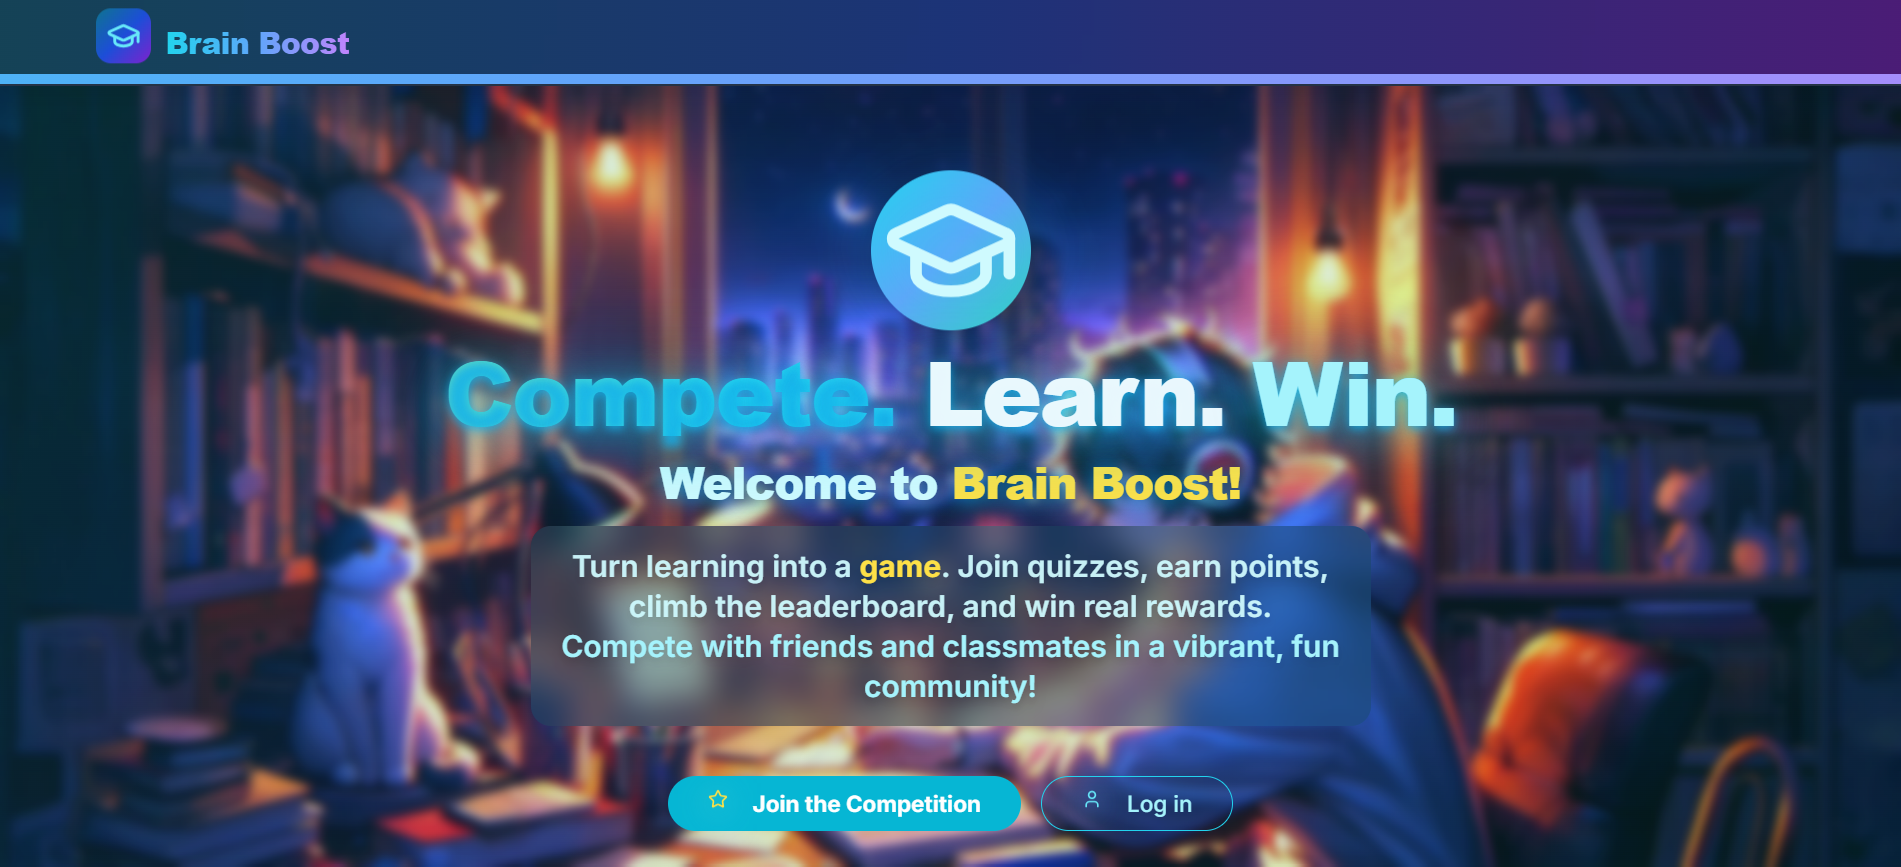
\includegraphics[width=0.8\textwidth]{screenshot/brainhome.png}
    \caption{\textbf{Accueil de l'application Brain Boost.} Interface d'accueil moderne et intuitive permettant l'accès aux principales fonctionnalités.}
\end{figure}

\begin{figure}[H]
    \centering
    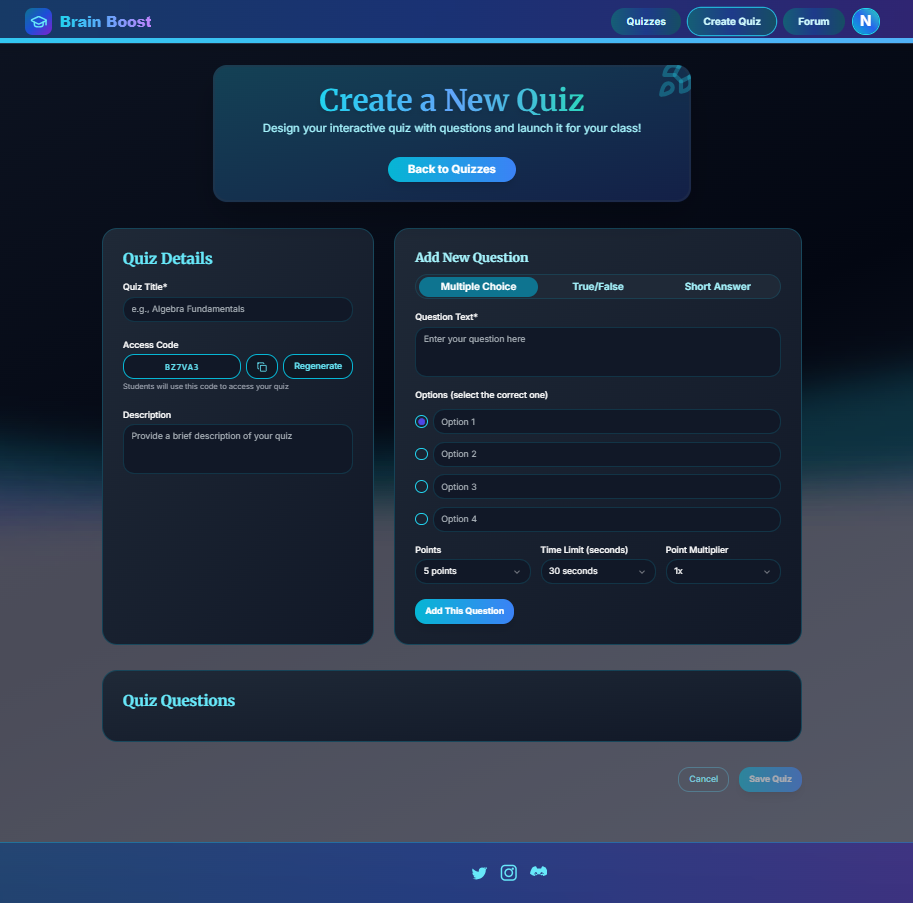
\includegraphics[width=0.8\textwidth]{screenshot/createquiz.png}
    \caption{\textbf{Création d'un quiz.} Espace dédié à la création de quiz personnalisés par l'enseignant, avec choix des questions et des paramètres.}
\end{figure}

\begin{figure}[H]
    \centering
    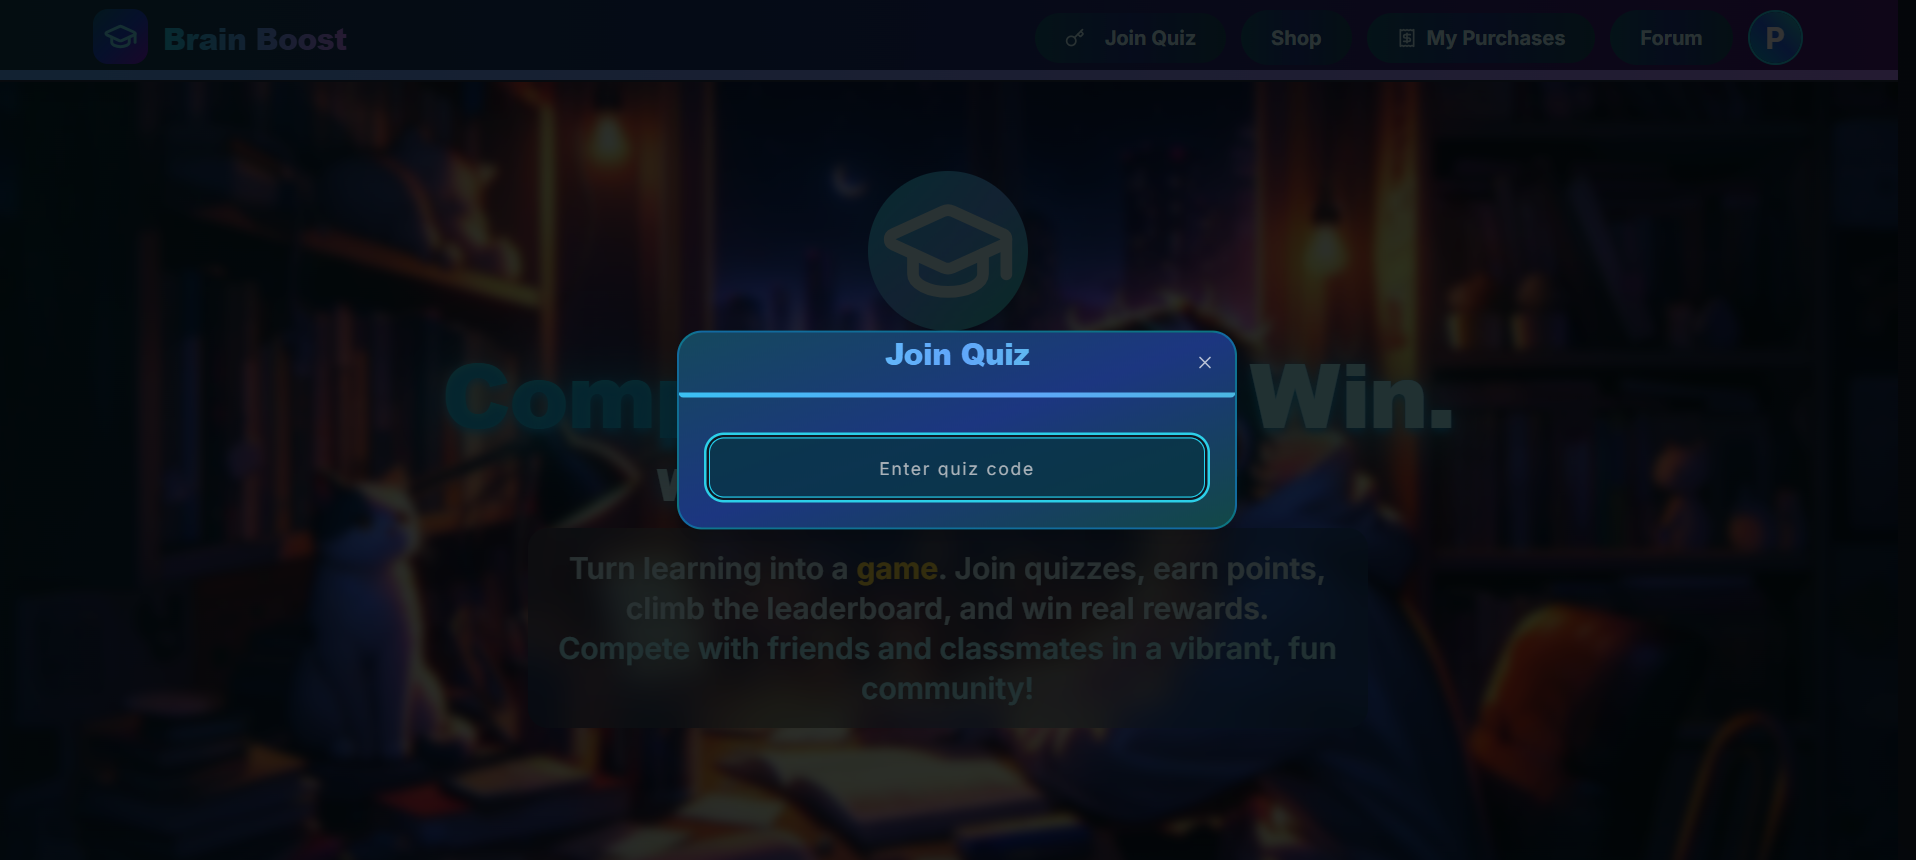
\includegraphics[width=0.8\textwidth]{screenshot/joinquiz.png}
    \caption{\textbf{Rejoindre un quiz.} Interface élève pour rejoindre une session de quiz en temps réel à l'aide d'un code d'accès.}
\end{figure}

\begin{figure}[H]
    \centering
    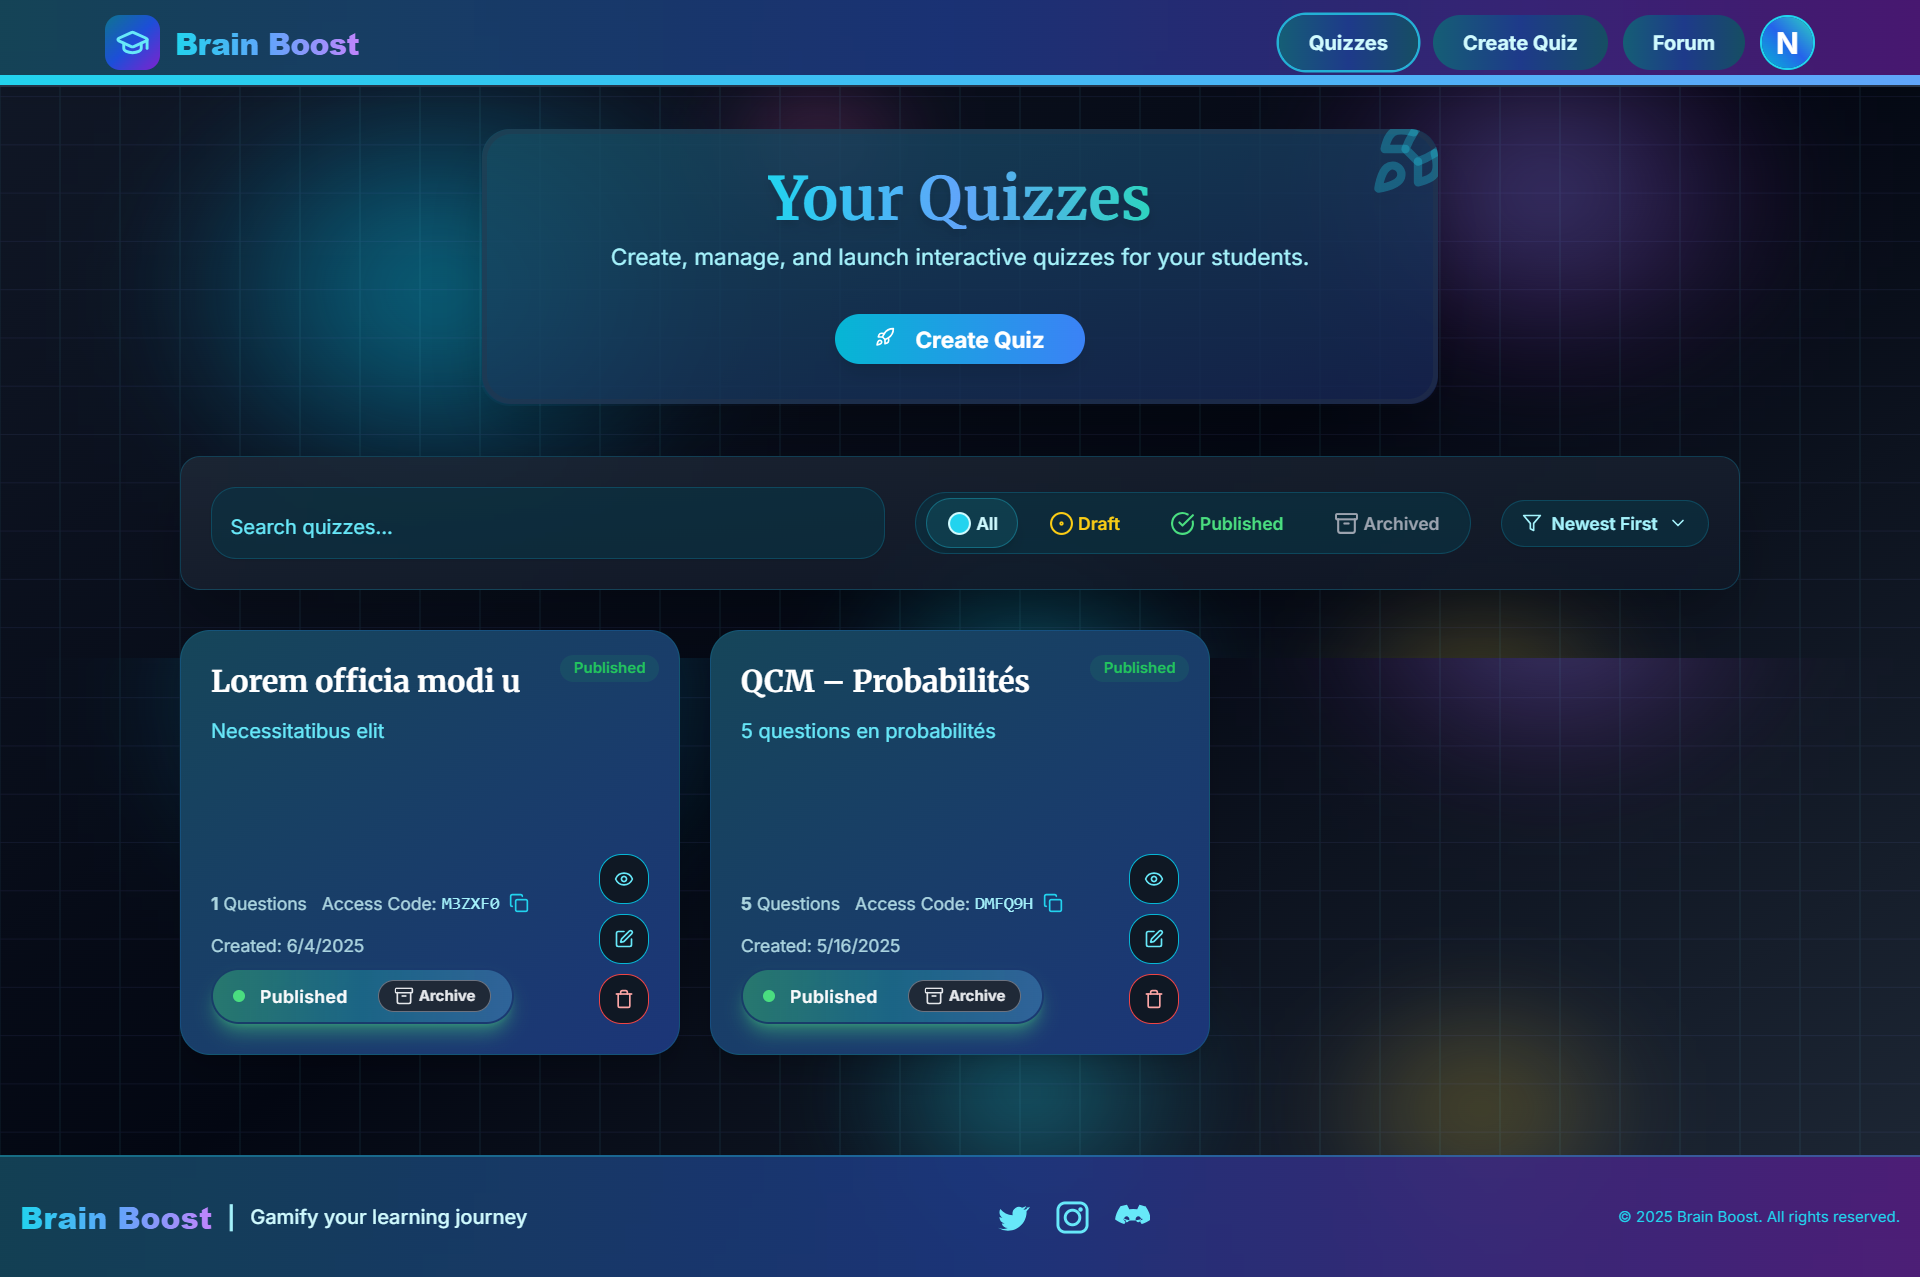
\includegraphics[width=0.8\textwidth]{screenshot/quiz.png}
    \caption{\textbf{Participation à un quiz.} Vue élève lors de la réponse aux questions d'un quiz en direct, avec feedback instantané.}
\end{figure}

\begin{figure}[H]
    \centering
    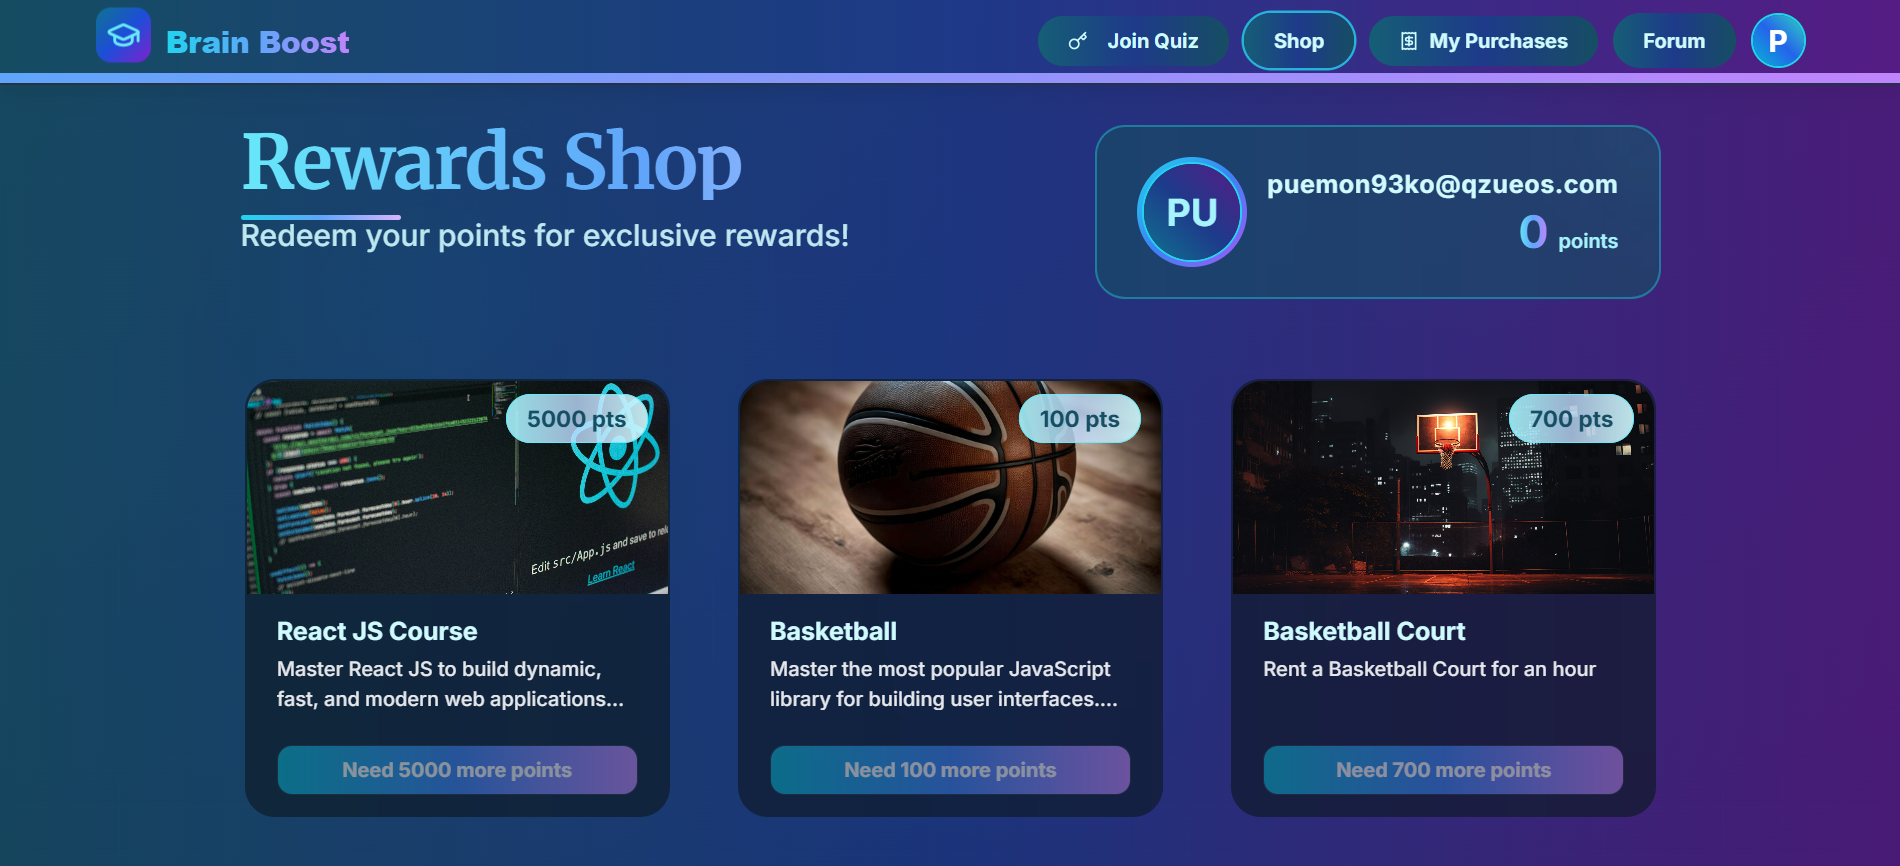
\includegraphics[width=0.8\textwidth]{screenshot/shop.png}
    \caption{\textbf{Boutique de récompenses.} Espace où les élèves peuvent échanger leurs points contre des thèmes, avatars ou autres personnalisations.}
\end{figure}

\begin{figure}[H]
    \centering
    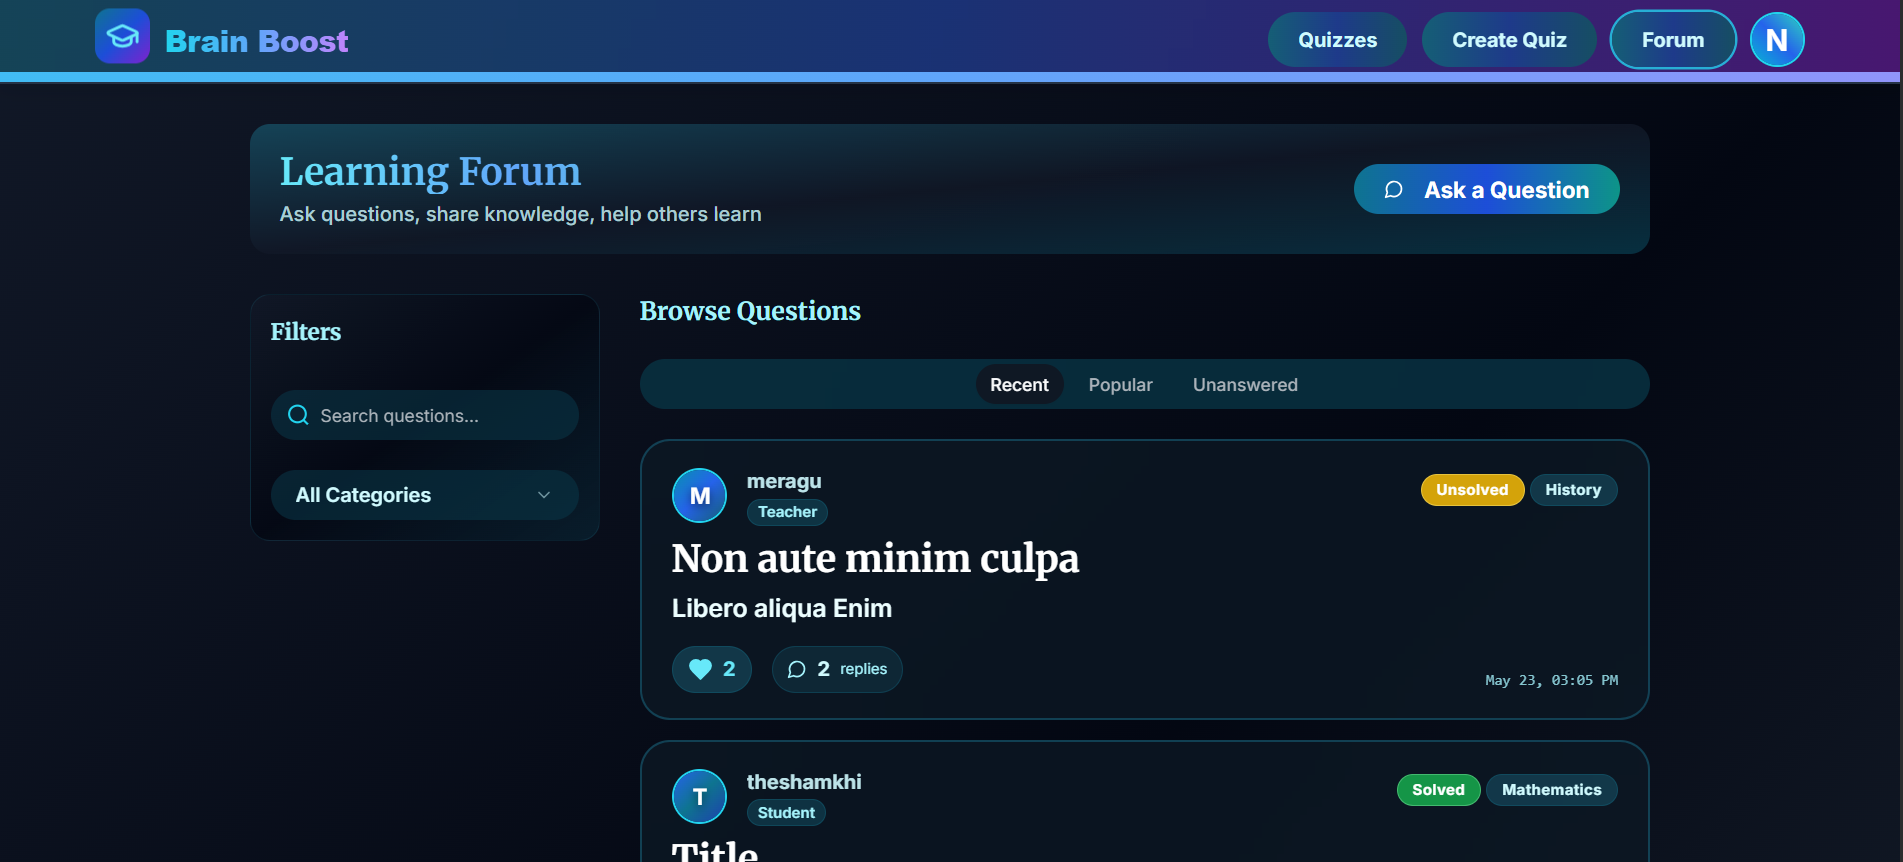
\includegraphics[width=0.8\textwidth]{screenshot/forum.png}
    \caption{\textbf{Forum collaboratif.} Plateforme d'entraide et de discussion où élèves et enseignants peuvent poser des questions, partager des astuces et interagir.}
\end{figure}

\begin{figure}[H]
    \centering
    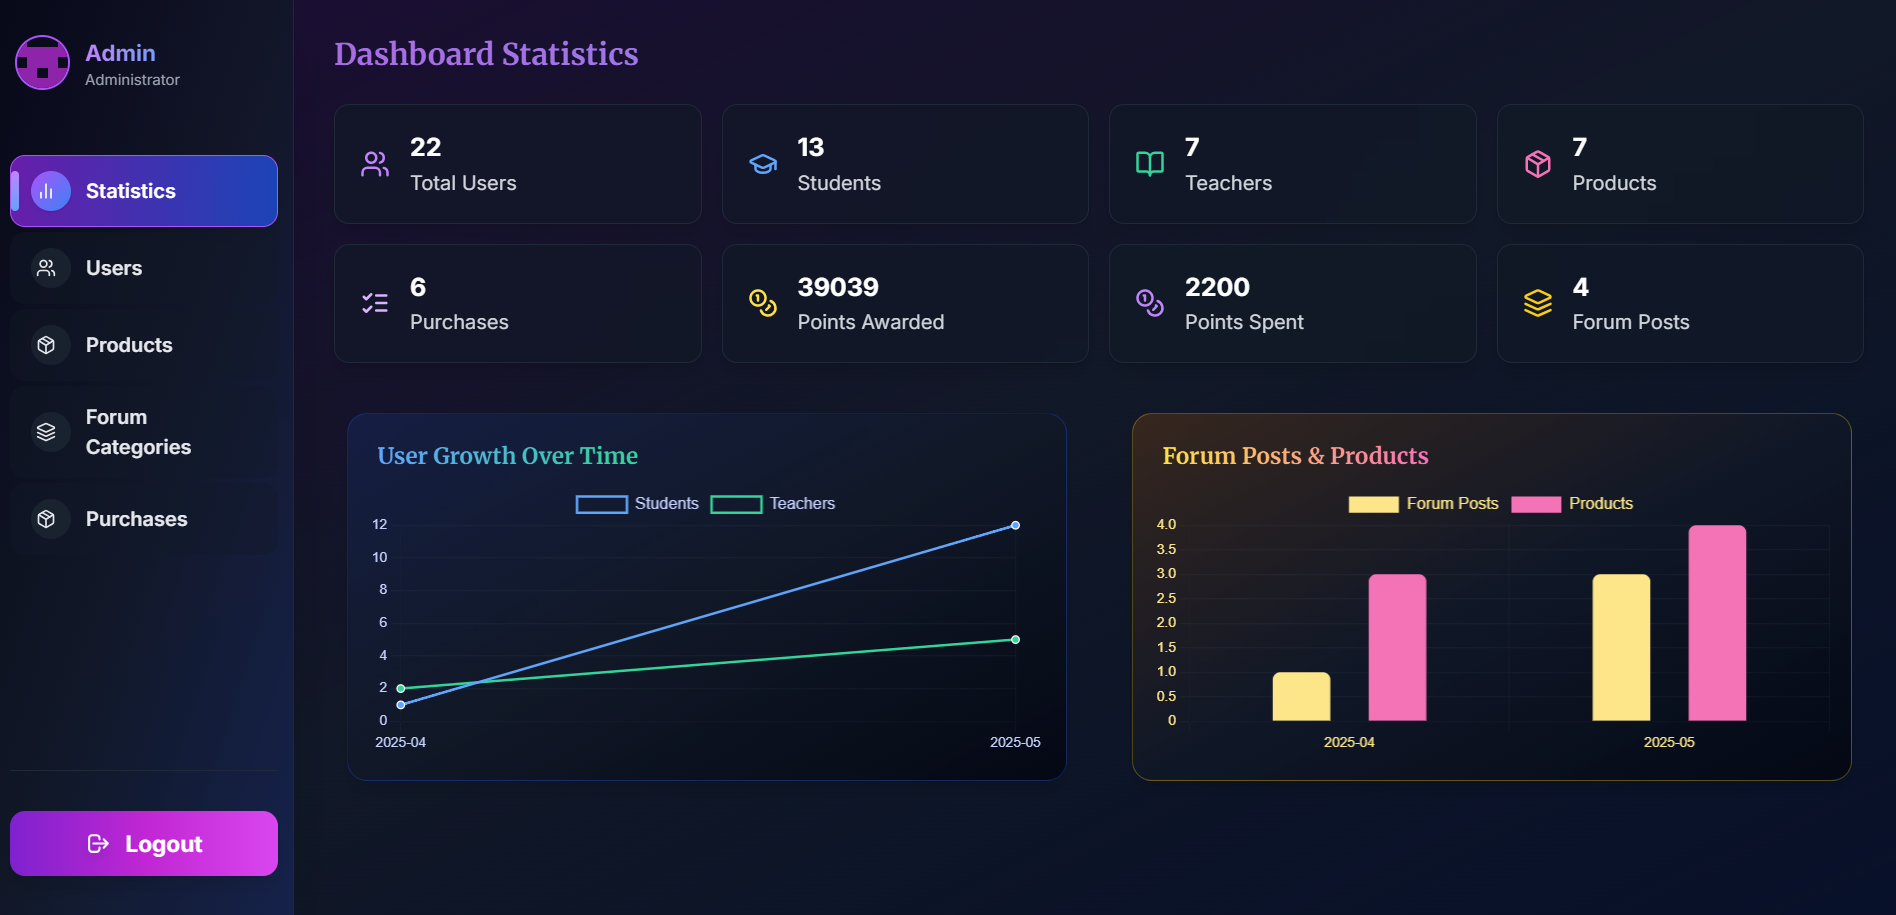
\includegraphics[width=0.9\textwidth]{screenshot/admin.png}
    \caption{\textbf{Tableau de bord administrateur.} Vue d'ensemble permettant à l'administrateur de visualiser toutes les statistiques de l'application et d'accéder, via la barre latérale, à la gestion des utilisateurs, de la boutique, du forum et des différentes sections de la plateforme.}
\end{figure}

\begin{figure}[H]
    \centering
    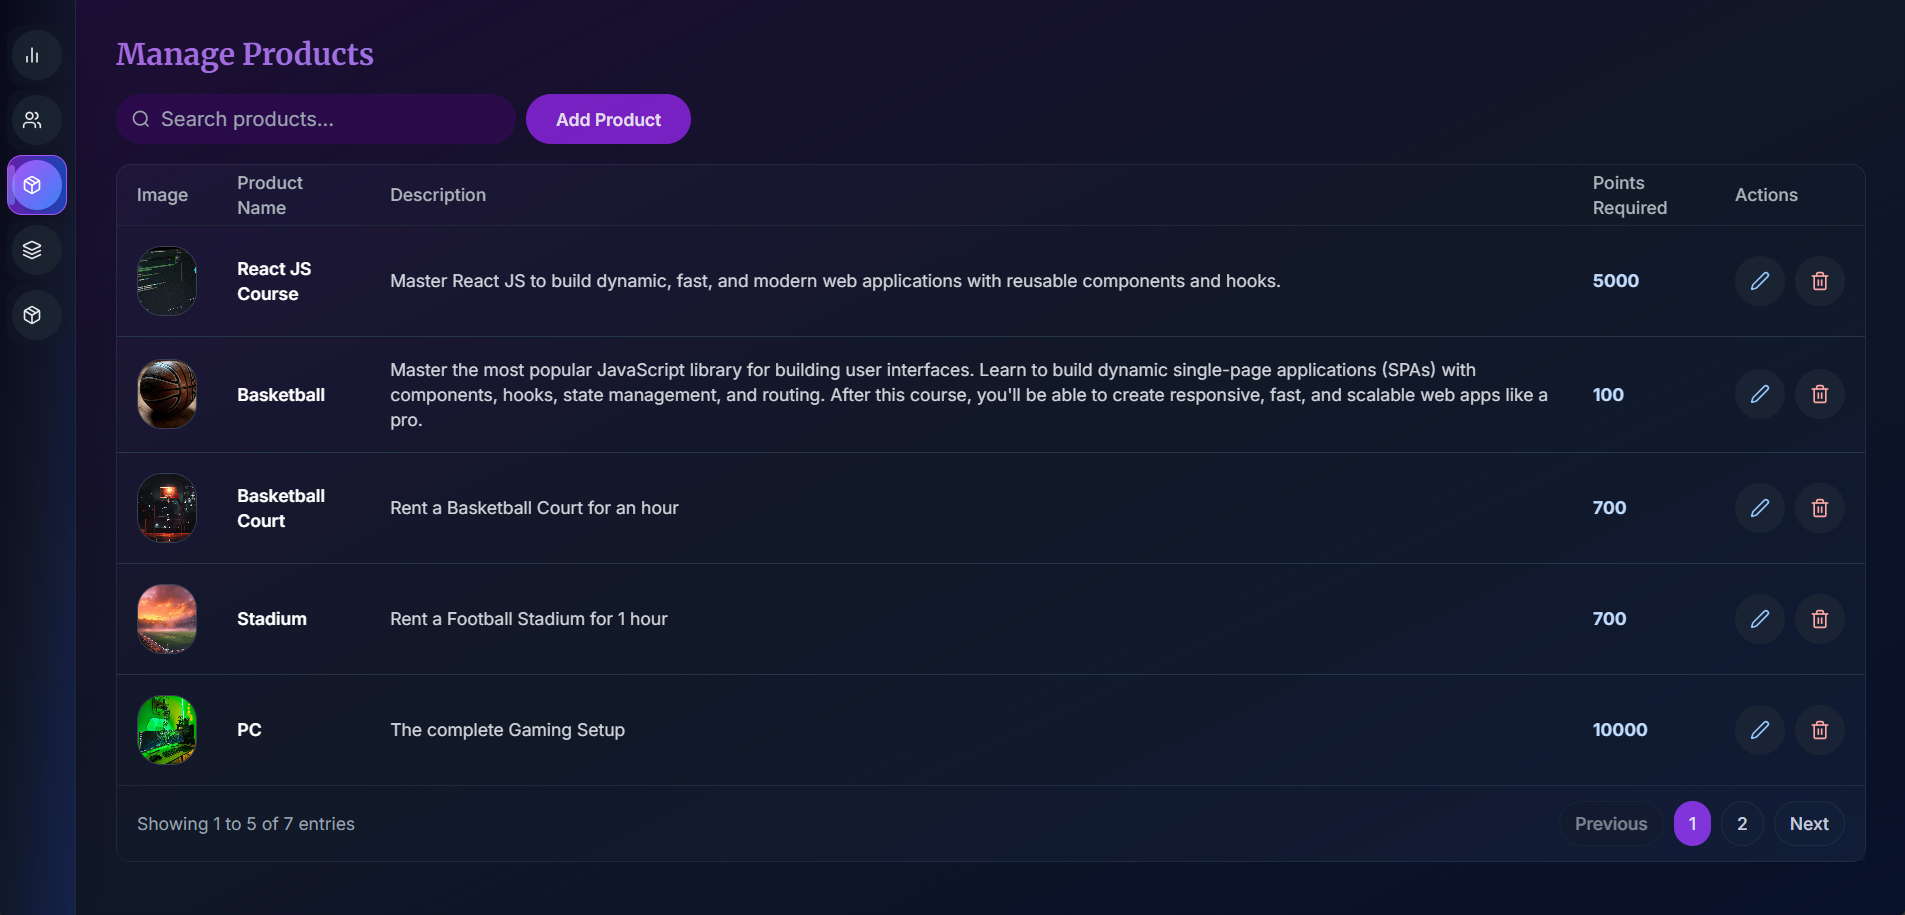
\includegraphics[width=0.8\textwidth]{screenshot/admin1.png}
    \caption{\textbf{Gestion des produits de la boutique (administrateur).} Tableau de gestion permettant à l'administrateur d'ajouter, modifier ou supprimer les produits disponibles dans la boutique de l'application.}
\end{figure}

\renewcommand{\bibname}{Bibliographie}
\begin{thebibliography}{99}

\bibitem{Belmadani2008}
Belmadani, A., et al. (2008). \textit{L'intégration des TIC dans l'enseignement secondaire au Maroc : état des lieux et perspectives}. Rabat : MEN.

\bibitem{Dillenbourg2019}
Dillenbourg, P. (2019). \textit{Orchestration Graphs: Modeling scalable education}. Lausanne : EPFL Press.

\bibitem{MEN2022}
Ministère de l'Éducation Nationale (MEN). (2022). \textit{Rapport sur l'intégration du numérique dans l'enseignement}. Rabat : MEN.

\bibitem{LIRADE2008}
LIRADE-TIE, Faculté des Sciences Ben M'Sik, Casablanca. (2008). \textit{Travaux et recherches sur l'intégration des TIC dans l'enseignement marocain}.

\bibitem{BonwellEison1991}
Bonwell, C. C., \& Eison, J. A. (1991). \textit{Active Learning: Creating Excitement in the Classroom}. ASHE-ERIC Higher Education Report No. 1. Washington, DC: George Washington University.


\end{thebibliography}
\end{document}